%\documentclass[14pt]{extreport}
\documentclass[12pt,a4paper]{report}
\usepackage[utf8]{vietnam}
\usepackage{amsmath, amsthm, amssymb}
\usepackage{enumerate}
\usepackage{verbatim}
\usepackage{fancyhdr}
\usepackage{pb-diagram}
\usepackage[all]{xy}  % Gói lệnh xy-pic
\usepackage[top=3.5cm, bottom=3cm, left=3.5cm, right=2cm]{geometry}
\usepackage{xcolor}
\usepackage{graphicx}
\usepackage{hyperref}
\makeatletter

%lenh them dong vao Mục lục
\def\them{\addcontentsline}


%Danh so Dinh li
\theoremstyle{definition}
\newtheorem{dl}{Định lý}
\newtheorem{corollary}{Hệ quả}
\newtheorem{lemma}{Bổ đề}
\newtheorem{md}{Mệnh đề}
\newtheorem{example}{Ví dụ}
\newtheorem*{cv}{Chứng minh}
\newtheorem{cy}{Chú ý}
\newtheorem{nx}{Nhận xét}
\newtheorem{vd}{Ví dụ}
\newtheorem{tc}{Tính chất}
\newtheorem{ql}{Quy luật}

\theoremstyle{definition}
\newtheorem{bt}{Bài toán}

\newtheorem{dn}{Định nghĩa}

\numberwithin{dl}{chapter}
\numberwithin{vd}{chapter}
\numberwithin{corollary}{chapter}
\numberwithin{lemma}{chapter}
\numberwithin{md}{chapter}
\numberwithin{dn}{chapter}
\numberwithin{cy}{chapter}
\numberwithin{nx}{chapter}

\newcommand{\vecto}{\overrightarrow}
\newcommand{\ct}{\uparrow \uparrow}
\newcommand{\Rn}{\mathbb{R}^n} 
\newcommand{\R}{\mathbb R}
\newcommand{\N}{\mathbb N} 
\newcommand{\si}{\sigma } 
\newcommand{\C}{\mathbb{C}} 
\newcommand{\Cn}{\mathbb{C}^n} 
\newcommand{\td}{\Leftrightarrow } 
\newcommand{\toi}{\longrightarrow }
\newcommand{\BA}{{\mathbb A}}
\newcommand{\BP}{{\mathbb P}}

\newcommand{\sr}{\Rightarrow } 
\newcommand{\Z}{\mathbb Z} 
\newcommand{\Zp}{\mathbb{Z}^p} 
\newcommand{\pr}{\mathbb{P}}
\newcommand{\dcong}{\partial }
\newcommand{\al}{\alpha}
\newcommand{\ga}{\gamma}
%\newcommand{\bt}{\beta}
\newcommand{\ld}{\lambda}
\newcommand{\ov}{\overline}

\newcommand{\Om}{\Omega}
\newcommand{\om}{\omega}
\newcommand{\dc}{(dd^c u)^n}

\newcommand{\m}[1]{
	\begin{bmatrix}
		#1
	\end{bmatrix}
}


\newcommand{\fs}[2]{\dfrac{#1}{#2}}
\newcommand{\di}{\displaystyle}

\DeclareMathOperator{\res}{res}
\DeclareMathOperator{\ind}{ind}
\DeclareMathOperator{\mult}{mult}
\DeclareMathOperator{\genus}{genus}
\DeclareMathOperator{\Id}{Id}


\usepackage{indentfirst}
%\newtheoremstyle{bt}% name
  %{3pt}%      Space above
%  {3pt}%      Space below
 % {}%         Body font
 % {}%         Indent amount (empty = no indent, \parindent = para indent)
 % {\bfseries}% Thm head font
  % {.}%        Punctuation after thm head
  % {.5em}%     Space after thm head: " " = normal interword space;
        %       \newline = linebreak
   % {}%  

 %\theoremstyle{bt}
 %\newtheorem{bt}{Bài}
% định nghĩa các lệnh tắt 
% định nghĩa các lệnh tắt 
 %\newcommand{\ebt}{\end{bt}}
 %định nghĩa các lệnh tắt 

 %\newcommand{\td}{\Leftrightarrow }
 %\newcommand{\sr}{\Rightarrow }
\def\them{\addcontentsline}
\makeatletter
\@addtoreset{vd}{sudsection}
\makeatother
%\renewcommand{mark}[1]
%{\mankright{}}
%\def\them\addcontensline
\renewcommand{\sectionmark}[1]
{\markright{\thesection\ \sl  #1}}
\lhead[\fancyplain{}{\thepage}]
{\fancyplain{}{\rightmark}}
\rhead[\fancyplain{}{\leftmark}]
{\fancyplain{}{\thepage}}
\cfoot{}


 
\begin{document}
\fontsize{13pt}{18pt}\selectfont % Lệnh thay đổi cỡ chữ thành cỡ 13, cỡ dòng 18(theo quy chuẩn của luận văn).

\setlength{\baselineskip}{17truept}

% =========Trang bìa ===================
\begin{titlepage}
\begin{center}
{\large\bf BỘ GIÁO DỤC VÀ ĐÀO TẠO}\\
{\large\bf TRƯỜNG ĐẠI HỌC SƯ PHẠM HÀ NỘI}\\
\vskip 5cm
{\large\bf TRƯƠNG THỊ CHUYÊN}\\
\vskip 3cm
{\Large\bf PHÂN TÍCH TÍNH CHẤT ỔN ĐỊNH \\ CỦA CÁC HỆ CHUYỂN MẠCH SUY BIẾN TUYẾN TÍNH VỚI HỆ SỐ HẰNG}
\vskip 3.5cm
{\large\bf LUẬN VĂN THẠC SĨ TOÁN HỌC}
 
\vskip 3.25cm

{\large\bf HÀ NỘI, 2022}
\end{center}
\end{titlepage}
\setcounter{page}{2}
\large 
%\newpage
\begin{titlepage}
\begin{center}
{\large\bf BỘ GIÁO DỤC VÀ ĐÀO TẠO}\\
{\large\bf TRƯỜNG ĐẠI HỌC SƯ PHẠM HÀ NỘI}\\
\vskip 4cm
{\large\bf TRƯƠNG THỊ CHUYÊN}\\
\vskip 3cm
{\Large \bf PHÂN TÍCH TÍNH CHẤT ỔN ĐỊNH  \\ CỦA CÁC HỆ CHUYỂN MẠCH SUY BIẾN \\ TUYẾN TÍNH VỚI HỆ SỐ HẰNG}
\vskip 1cm

\begin{tabular}{r l}
\textit{\large\bf Chuyên ngành:}&{\large\bf Toán Ứng dụng}\\
\textit{\large\bf Mã số:}&\large\bf 8 46 01 12\\
\end{tabular}

\vskip 2cm
{\large\bf LUẬN VĂN THẠC SĨ TOÁN HỌC}\\
\vskip 1.5cm
{\large\bf Người hướng dẫn khoa học: TS. Hà Phi}\\
\vskip 1.2cm

 {\large\bf HÀ NỘI, 10 - 2022}\\
\end{center}
\end{titlepage}


\tableofcontents

\setlength{\baselineskip}{0.75cm}
\chapter*{\centerline{Lời cảm ơn}} \them{toc}{chapter}{Lời cảm ơn}
\markboth{ Lời cảm ơn}{ Lời cảm ơn}%tieu de chay cho Loi cảm ơn

Tôi xin chân thành cảm ơn các thầy cô trong Bộ môn Toán ứng dụng, Trường Đại học Sư phạm Hà Nội đã giúp đỡ tôi trong quá trình học tập cũng như trong quá trình hoàn thành luận văn này.

Đặc biệt, tôi xin gửi lời cảm ơn chân thành và sâu sắc đến TS.Hà Phi, người đã tận tâm hướng dẫn và giúp đỡ tôi trong quá trình làm luận văn để luận văn này.

Cuối cùng tôi xin gửi lời cảm ơn tới gia đình, người thân, bạn bè, và các bạn trong nhóm Toán ứng dụng đã có rất nhiều giúp đỡ và góp ý cho tôi trong quá trình học tập cũng như làm luận văn.

\indent Do hạn chế về khả năng, thời gian thực hiện nên luận văn không tránh khỏi những thiếu sót. Vì vậy tôi rất mong nhận được những ý kiến đóng góp của thầy cô và các bạn.
\vskip 1cm
\qquad \qquad \qquad \qquad \qquad \qquad\qquad Hà Nội, tháng 10 năm 2022
\vskip 0.5cm
\qquad \qquad \qquad \qquad \qquad \qquad \qquad \qquad  \qquad \qquad Tác giả \\
\\
\vskip 0.5cm
\qquad \qquad \qquad \qquad \qquad \qquad \qquad  \qquad \quad \quad Trương Thị Chuyên

\chapter*{\centerline{Lời cam đoan}} \them{toc}{chapter}{Lời cam đoan}
\markboth{ Lời cam đoan}{ Lời cam đoan}%tieu de chay cho Loi cam đoan
Tôi xin cam đoan bản luận án này là kết quả nghiên cứu của cá nhân tôi. Các số liệu và tài liệu được trích dẫn trong luận án là trung thực. Kết quả nghiên cứu này không trùng với bất cứ công trình nào đã được công bố trước đó. 

Tôi chịu trách nhiệm với lời cam đoan của mình.

\vskip 1cm
\qquad \qquad \qquad \qquad \qquad \qquad \qquad  Hà Nội, tháng 10 năm 2022
\vskip 0.5cm
\qquad \qquad \qquad \qquad \qquad \qquad \qquad \qquad \qquad \qquad Tác giả \\
\\
\vskip 0.5cm
\qquad \qquad \qquad \qquad \qquad  \quad \quad \qquad \qquad  \qquad  Trương Thị Chuyên

\newpage

\chapter*{Lời nói đầu}\them{toc}{chapter}{Lời nói đầu}
\markboth{ Lời nói đầu}{ Lời nói đầu}%tieu de chay cho Loi nói đầu
%\textbf{1. Lý do chọn đề tài}\\
Trong những năm gần đây, việc phân tích tích chất ổn định và thiết kế bộ điều khiển cho các hệ thống chuyển mạch đã thu hút được rất nhiều sự quan tâm của các nhà nghiên cứu trong và ngoài nước. 
Hệ thống chuyển mạch xuất hiện trong nhiều ứng dụng, chẳng hạn như hệ thống điện/điện tử, hệ thống điều khiển chuyến bay, hệ thống điều khiển mạng, điều khiển robot, hệ thống kinh tế, v.v. 
Động lực để nghiên cứu các hệ thống chuyển mạch đến từ việc một hệ thống thực tế có thể bao gồm nhiều hệ thống con phụ thuộc vào các yếu tố môi trường khác nhau (các tham số môi trường).
Bên cạnh đó, các phương pháp thiết kế điều khiển thông minh được phát triển dựa trên ý tưởng chuyển đổi giữa các bộ điều khiển khác nhau. 
Do đó, nghiên cứu về hệ thống chuyển mạch đóng góp rất lớn trong việc thiết kế bộ điều khiển chuyển mạch và bộ điều khiển thông minh.

Bên cạnh các hệ chuyển mạch thì các hệ thống suy biến (hay còn gọi là các phương trình vi phân/sai phân ẩn, phương trình vi phân đại số) có vai trò vô cùng quan trọng trong lĩnh vực toán ứng dụng/toán công nghiệp. So với các mô hình không gian trạng thái cổ điển, việc nghiên cứu hệ thống suy biến khó khăn hơn, bởi vì bên cạnh tích chất ổn định ta còn phải xem xét đồng thời tính chính quy và tính khử xung (đối với trường hợp thời gian liên tục) và quan hệ nhân quả (đối với trường hợp thời gian rời rạc). 

Mặc dù các hệ thống chuyển mạch cũng như các hệ thống suy biến đã được nghiên cứu rất mạnh từ năm 1990 trở lại đây, nhưng lớp các hệ giao thoa giữa chúng (được gọi là các hệ chuyển mạch suy biến) mới chỉ được quan tâm nghiên cứu từ năm 2012 cho đến nay. Với mong muốn được tìm hiểu kĩ hơn về tính chất ổn định của hệ các hệ chuyển mạch suy biến và ứng dụng trong thực tế, tôi quyết định chọn đề tài \textbf{``Phân tích tính chất ổn định của các hệ chuyển mạch suy biến tuyến tính với hệ số hằng''} cho luận văn thạc sĩ của mình. 

Hai vấn đề cơ bản được quan tâm trong luận văn này là:\\
i) Nghiên cứu về tính chất ổn định của hệ chuyển mạch dưới quy luật chuyển mạch bất kỳ, đặc biệt trong trường hợp các hệ con là ổn định. \\
ii) Thiết kế quy luật chuyển mạch để ổn định hóa hệ tổng, đặc biệt trong trường hợp các hệ con là không ổn định.

Đối tượng được quan tâm đến trong luận văn đó là lớp các hệ chuyển mạch suy biến có dạng
%
\[
E \dot{x}(t) = A_{\sigma(t)} x(t), 
\]
%
trong đó $\sigma: \mathbb{R}_+ \longrightarrow \{1,\ 2, ..., N \}$ thể hiện tín hiệu chuyển mạch. Ở đây $E$ là một ma trận suy biến (tức là $\det(E)=0$).\\

\vskip 0.5cm
\qquad \qquad \qquad \qquad \qquad \qquad \qquad  Hà Nội, ngày  tháng  năm 2022

\newpage
\addcontentsline{toc}{chapter}{Danh mục kí hiệu}

\chapter*{Danh mục kí hiệu}
	\begin{table}[!h]
			\begin{tabular}{lll}
			\hline 
			Kí hiệu  & Ý nghĩa \\ 
			\hline
                $\mathbb{R}^{n}$ &  Tập các vector thực $n$ chiều\\
			    $\mathbb{R}^{n \times m}$ &  Tập các ma trận thực $n \times m$ chiều\\
                $x^{T}$ & Vector chuyển vị của vector $x$\\
                $I_{n}$ & Ma trận đơn vị $n \times n$ chiều\\
                $V^{T}$ & Ma trận chuyển vị của ma trận $V$\\
                $A^{-1}$ & Ma trận nghịch đảo của ma trận $A$\\
                $\operatorname{rank} E$ & Hạng của ma trận $E$\\
			det(A)  &  Định thức của ma trận vuông A \\ 	
			Null $E$  & Hạt nhân của ma trận $E$ , \\
		\hline 
		\end{tabular} 
\end{table}

\chapter{Kiến thức chuẩn bị}\label{Chapter 1}

\section{Sơ lược về hệ chuyển mạch không suy biến}\label{Section 1.1}

Trong mục này ta sẽ đi tìm hiểu một ví dụ ứng dụng của hệ thống chuyển mạch trong
kỹ thuật và tính chất ổn định của hệ thống tuyến tính không suy biến.

\begin{vd}
Trong ví dụ này, mô hình của bộ chuyển đổi tăng áp PWM được xây dựng dưới dạng một hệ thống chuyển mạch, xem \cite{book1}. Bộ chuyển đổi tăng áp đã được áp dụng trong nhiều hệ thống điện tử khác nhau, với đặc điểm chính là nó chỉ có ba biến điều khiển, tức là $1$, $-1$ và $0$. Hình \ref{fig:screenshot005} cho thấy sơ đồ của một bộ chuyển đổi tăng áp và Hình \ref{fig:screenshot006} cho thấy một phương pháp điều khiển hai biến chỉ bao gồm 0 và 1. 

\begin{figure}[h!]
	\centering
	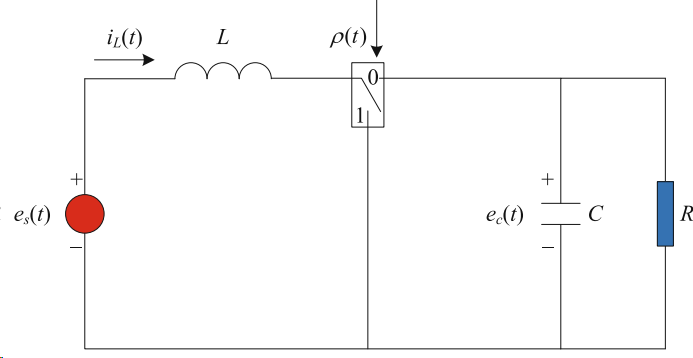
\includegraphics[width=0.8\linewidth]{screenshot005}
	\caption{Sơ đồ mạch điện của bộ chuyển đổi tăng áp}
	\label{fig:screenshot005}
\end{figure}

\begin{figure}[h!]
	\centering
	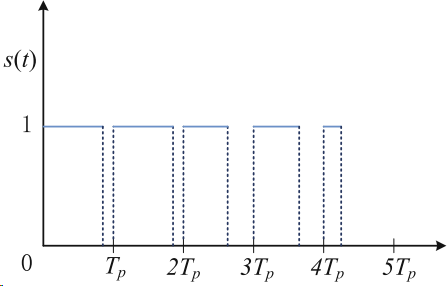
\includegraphics[width=0.8\linewidth]{screenshot006}
	\caption{Tín hiệu chuyển mạch $s(t)$}
	\label{fig:screenshot006}
\end{figure}

\noindent Trong Hình \ref{fig:screenshot005}, L là cuộn cảm, C là tụ điện, R là điện trở tải, $e_s(t)$ là nguồn. Giá trị của công tắc $s(t)$ được kích hoạt bởi thiết bị PWM. Giả sử rằng chu kỳ của PWM là $T_p$ và công tắc $s(t)$ chỉ có thể chuyển đổi một lần trong một chu kỳ, độ rộng của PWM có thể được mô tả bằng một trong Hình\ref{fig:screenshot006}. 
Bằng việc giới thiệu các biến $\tau = t / T_p$, $L_1 = L / T_p$ và $C_1 = C / T_p$, $s(t) \in \{0,1\}$. Ta xét tín hiệu chuyển mạch $\si(t) = s(t)+1$ và đặt 
$x_1 = e_c$, $x_2 = i_L$, $u = e_s$, thì mô hình động lực học của bộ biến đổi tăng áp có thể được mô tả bằng hệ điều khiển chuyển mạch sau:
%
\begin{equation}
\dot{x}(t) = A_{\si(t)} x(t) + B_{\si(t)} u(t),     
\end{equation}
%
trong đó $\si(t) \in \{1,2\}$ với mọi $t\geq 0$.\\
%
Bằng việc thiết kế tín hiệu chuyển mạch phù hợp để sử dụng cả hai hệ con (tương ứng với 2 giá trị $1$, $2$ của tín hiệu chuyển mạch $\si(t)$), ta có thể đạt được một tính chất nào đó của hệ, ví dụ như tính ổn định, tính tiêu tán, v.v .
\end{vd}

Để có thể phân tích về tính chất ổn định của các hệ tuyến tính chuyển mạch, sau đây ta sẽ đi nhắc lại ngắn gọn tính chất ổn định của hệ tuyến tính (không chuyển mạch) sau
%
\begin{equation}\label{1.0}
\dot{x}(t)=A x(t), 
\end{equation}
%
trong đó $x(t) \in \mathbb{R}^{n}, A \in \mathbb{R}^{n \times n}$. Hệ \eqref{1.0} được gọi là \textbf{ổn định mũ} nếu nghiệm của nó thỏa mãn đánh giá
%
\[
\|x(t)\| \leq Ce^{-\gamma t}, \mbox { với mọi } t\geq 0,
\]
%
với các hằng số dương $C$ và $\gamma$ nào đó. Tương tự như vậy, hệ rời rạc
%
\begin{equation}\label{1.22}
x(k+1) = A x(k)
\end{equation}
%
được gọi là \textbf{ổn định mũ} nếu nghiệm của nó thỏa mãn đánh giá
%
\[
\|x(k)\| \leq Ce^{-\gamma k}, \mbox { với mọi } k \in \mathbb{N},
\]
%
với các hằng số dương $C$ và $\gamma$ nào đó.

\begin{md}
i) Hệ \eqref{1.0} là ổn định mũ khi và chỉ khi tất cả các giá trị riêng của A có phần thực âm thực sự. Khi đó ma trận $A$ được gọi là \textbf{ổn định Hurwitz}. \\
ii) Hệ \eqref{1.22} là ổn định mũ khi và chỉ khi tất cả các giá trị riêng của A có modulo thực sự nhỏ hơn $1$. Khi đó ma trận $A$ được gọi là \textbf{ổn định Schur}.
\end{md} 

Một ma trận P đối xứng được gọi là xác định dương (kí hiệu $P > 0$) nếu $x^TPx > 0\quad \forall x \neq 0.$ Tiếp theo, ta sẽ nhắc lại khái niệm hàm Lyapunov.

\begin{dl} 
i) Ma trận $A$ của hệ \eqref{1.0} là ổn định Hurwitz khi và chỉ khi với mọi ma trận $Q=Q^{T}>0$, tồn tại một ma trận $P=P^{T}>0$ sao cho phương trình Lyapunov liên tục sau được thỏa mãn
%
\begin{equation}\label{LMI}
A^{T} P+P A=-Q \ .
\end{equation}
Hàm $V(x):=x^{T} P x$ khi đó được gọi là hàm Lyapunov liên kết với hệ.\\
ii) Ma trận $A$ của hệ \eqref{1.0} là ổn định Schur khi và chỉ khi với mọi ma trận $Q=Q^{T}>0$, tồn tại một ma trận $P=P^{T}>0$ sao cho phương trình Lyapunov rời rạc sau được thỏa mãn
%
\begin{equation}\label{LMI}
A P A^{T} - P = - Q \ .
\end{equation}
\end{dl}

Như vậy, điều kiện đủ cho tính ổn định mũ của phương trình \eqref{1.0} có thể được kiểm tra bằng cách giải bất đẳng thức ma trận tuyến tính (LMI) \eqref{LMI} với ẩn số $P$.


\section{Sơ lược về hệ suy biến tuyến tính}
Trong mục này ta tìm hiểu sơ lược về các hệ suy biến tuyến tính trong trường hợp thời gian liên tục
\begin{equation}\label{1.1}
E\dot{x}(t)=A x(t),
\end{equation}
hoặc trường hợp thời gian rời rạc 
\begin{equation}\label{1.2}
\operatorname{E}x(k+1)=A x(k),
\end{equation}
%
trong đó $t \in \mathbb{R}$ biểu thị thời gian liên tục, số nguyên không âm $k$ biểu thị thời gian rời rạc, $x(t)(x(k)) \in \mathbb{R}^{n}$ là biến, $E, A \in \mathbb{R}^{n \times n}$ là các ma trận hằng. Ma trận $E$ có thể suy biến, tức là $\det(E)=0$ hay hạng của ma trận $E$ là $\operatorname{rank} E = r < n$.

Nếu $\det(sE-A) \not \equiv 0$ hoặc $\det(zE-A) \not \equiv 0$, hệ tuyến tính \eqref{1.1} hoặc \eqref{1.2} có nghiệm duy nhất với điều kiện ban đầu tương thích và được gọi là chính quy. Các giá trị riêng hữu hạn của cặp ma trận  $(E, A)$ là các nghiệm của phương trình đặc trưng $\det(sE-A)=0$ hoặc $\det(zE-A)=0$. Nếu các giá trị riêng hữu hạn nằm ở nửa mặt phẳng bên trái của $s$ (đĩa đơn vị mở của $z$) thì nghiệm giảm dần theo cấp số nhân. Các giá trị riêng vô hạn của  $(E, A)$ với các vector riêng thỏa mãn ràng buộc đại số của hệ, như sẽ thấy ở hệ phương trình \eqref{1.6} và \eqref{1.7} phía dưới.\\

\begin{dn} 
i) Hệ thống \eqref{1.1} (tương ứng \eqref{1.2}) được gọi là không có xung nếu thỏa mãn điều kiện $\operatorname{rank} E=\operatorname{deg}(\det(sE-A))$ (tương ứng $\operatorname{deg}(\det(zE-A)$). \\
ii) Hệ thống \eqref{1.1} (tương ứng \eqref{1.2}) được gọi là ổn định mũ nếu như nó là chính quy và nghiệm của nó thỏa mãn đánh giá
%
\[
\|x(t)\| \leq Ce^{-\gamma t}, \mbox { với mọi } t\geq 0,
\]
%
hoặc 
%
\[
\|x(k)\| \leq Ce^{-\gamma k}, \mbox { với mọi } k \in \mathbb{N},
\]
%
với các hằng số dương $C$ và $\gamma$.
\end{dn}


\begin{lemma}\label{bd1.1} (Phân rã Weiertrass, \cite{LTW11}) \\
i) Nếu hệ \eqref{1.1} hoặc \eqref{1.2} là chính quy thì tồn tại hai ma trận khả nghịch  $M$ và $N$ sao cho 
%
\begin{equation}\label{1.3}
M E N=\left[\begin{array}{cc}I_{d} & 0 \\ 0 & J\end{array}\right],\ M A N=\left[\begin{array}{cc}\Lambda & 0 \\ 0 & I_{n-d}\end{array}\right]
\end{equation}
%
trong đó $d=\operatorname{deg}(\det(sE-A))$ hoặc $d=\operatorname{deg}\det(zE-A))$. $J$ được tạo thành từ các khối Jordan tương ứng giá trị riêng không.\\
ii) Nếu hệ \eqref{1.1} hoặc \eqref{1.2} chính quy và không có xung thì $d=r$ hoặc trong \eqref{1.3} ta có $J=0$. \\
iii) Nếu hệ \eqref{1.1} (hoặc \eqref{1.2}) ổn định thì $\Lambda$ là ổn định Hurwitz (Schur).
\end{lemma}
Cho phân tích giá trị kì dị (SVD) của $E$ là
\begin{equation}\label{1.4}
E=U\left[\begin{array}{cc}
E_{11} & 0 \\
0 & 0
\end{array}\right] V^{T}, E_{11}=\operatorname{diag}\left\{\sigma_{1}, \ldots, \sigma_{r}\right\} \\
\end{equation}
trong đó $\sigma_{1} \geq \sigma_{2 } \geq \ldots \geq \sigma_{r}$ , $U$ và $V$ là ma trận trực chuẩn $\left(U^{T} U=V^{T} V=I\right)$. Đặt
\begin{equation}\label{1.5}
\bar{x}=V^{T} x \triangleq\left[\begin{array}{c}
\bar{x}_{1} \\
\bar{x}_{2}
\end{array}\right],\ U^{T} A V=\left[\begin{array}{ll}
A_{11} & A_{12} \\
A_{21} & A_{22}
\end{array}\right], \\
\end{equation}
thì phương trình vi phân (sai phân) trong  \eqref{1.1}hoặc \eqref{1.2} có dạng
\begin{equation}\label{1.6}
\begin{aligned}
E_{11} \dot{\bar{x}}_{1}(t) &=A_{11} \bar{x}_{1}(t)+A_{12} \bar{x}_{2}(t), \\
0 &=A_{21} \bar{x}_{1}(t)+A_{22} \bar{x}_{2}(t)
\end{aligned} \\
\end{equation}
hoặc
\begin{equation}\label{1.7}
\begin{aligned}
E_{11} \bar{x}_{1}(k+1) &=A_{11} \bar{x}_{1}(k)+A_{12} \bar{x}_{2}(k), \\
0 &=A_{21} \bar{x}_{1}(k)+A_{22} \bar{x}_{2}(k).
\end{aligned} \\
\end{equation}
Từ những điều trên, có thể dễ dàng nhận ra rằng hệ là chính quy và không có xung khi và chỉ khi $A_{22}$ khả nghịch. Hơn nữa, hệ ổn định khi và chỉ khi $A_{22}$ khả nghịch và  $E_{11}^{-1}\left(A_{11}-A_{12} A_{22}^{-1} A_{21}\right)$ là ổn định Hurwitz (hoặc Schur).


\section{Phát biểu bài toán}\label{Section 1.3}

Xét hệ chuyển mạch bao gồm $\mathcal{N}$ hệ con tuyến tính thời gian liên tục. 
\begin{equation}\label{1.8}
E \dot{x}(t)=A_{i} x(t), \\
\end{equation}
hoặc $\mathcal{N}$ hệ con tuyến tính thời gian rời rạc
\begin{equation}\label{1.9}
E x(k+1)=A_{i} x(k), \\
\end{equation}
trong đó vector $x \in \mathbb{R}^{n}$ và ma trận  $E$ cũng như trong \eqref{1.1} và \eqref{1.2}. Chỉ số $i$ biểu thị hệ con thứ $i$ và nhận giá trị trong tập rời rạc $\mathcal{I}=\{1,2, \ldots, \mathcal{N}\}$. Cặp ma trận $(E,A_{i})$ là đại diện cho động lực học của hệ con thứ i.

Cho một quy luật chuyển mạch, hệ chuyển mạch \eqref{1.8} ( hoặc \eqref{1.9}) được gọi là ổn định nếu bắt đầu từ bất kỳ giá trị ban đầu nào, hệ đều hội tụ đến điểm gốc.

\begin{nx}\label{Nx1} Có một giả định ngầm trong hệ chuyển mạch được mô tả bởi \eqref{1.8} và \eqref{1.9} là ma trận mô tả  $E$ là chung cho tất cả hệ con. Về mặt lý thuyết, giả định này là hạn chế ở hiện tại. Tuy nhiên, như đã thảo luận trong \cite{Zhai09a} , có một số giải pháp có thể được áp dụng cho các hệ tuyến tính đơn. Đây là lý do chính tại sao ta hiện đang xem xét ma trận mô tả chung $E$ trong hệ chuyển mạch. Ví dụ, nếu cho một hệ duy nhất 
$$
E \dot{x}(t)=A x(t)+B u(t)
$$
$(E x(k+1)=A x(k)+B u(k))$, trong đó $u(t)$ $(u(k))$ là đầu vào điều khiển, ta có thể thiết kế hai bộ mô tả ổn định phản hồi thay đổi $u=K_{1} x, u=K_{2} x$. Hơn nữa, hệ bao gồm các hệ con được đặc trưng bởi $\left(E, A+B K_{1}\right)$ và $\left(E, A+B K_{2}\right)$ là ổn định dưới quy luật chuyển mạch tùy ý. Sau đó, ta có thể chuyển mạch tùy ý giữa hai bộ điều kiển và do đó xem xét thông số kỹ thuật điều khiển cao hơn.\\
\end{nx}
Trong thực tế, hệ tuyến tính chuyển mạch có thể không ổn định ngay cả khi tất cả các hệ con đều ổn định. Một ví dụ minh họa dựa trên tài liệu tham khảo \cite{Br98} được đưa ra như sau.\\
%
\begin{vd}  Xét một hệ chuyển mạch bao gồm hai hệ tuyến tính con có ma trận là:\\
$$
\begin{aligned}
E =\left[\begin{array}{ccc}
1 & 0 & 0 \\
0 & 1 & 0 \\
0 & 0 & 0
\end{array}\right], \
A_{1}= {\left[\begin{array}{ccc}
-1 & 10 & 0 \\
-100 & -1 & 0 \\
0 & 0 & 1
\end{array}\right] }, \   
A_{2}= {\left[\begin{array}{ccc}
-1 & 100 & 0 \\
-10 & -1 & 0 \\
0 & 0 & 1
\end{array}\right] }.
\end{aligned} 
$$
Ta viết lại hai hệ $E\dot{x}=A_{i}x$, $i=1,2$, như sau

$$
\begin{array} { l } 
{ {\left[\begin{array}{cc}
1 & 0 \\
0 & 1 
\end{array}\right] }{\left[\begin{array}{cc}
\dot{x} _ { 1 } \\
\dot{x} _ { 2 }
\end{array}\right] } = {\left[\begin{array}{cc}
-1 & 10 \\
-100 & -1 
\end{array}\right] } } {\left[\begin{array}{cc}
x _ { 1 } \\
x _ { 2 }
\end{array}\right] }\\
{ x _ { 3 } = 0 }
\end{array}
$$
và
$$
\begin{array} { l } 
{ {\left[\begin{array}{cc}
1 & 0 \\
0 & 1 
\end{array}\right] }{\left[\begin{array}{cc}
\dot{x} _ { 1 } \\
\dot{x} _ { 2 }
\end{array}\right] } = {\left[\begin{array}{cc}
-1 & 100 \\
-10 & -1 
\end{array}\right] } } {\left[\begin{array}{cc}
x _ { 1 } \\
x _ { 2 }
\end{array}\right] }\\
{ x _ { 3 } = 0 }
\end{array}.
$$
Rõ ràng, $x_{3}$ trong cả hai hệ đều bằng không do ràng buộc phương trình đại số, và cặp  $\left(x_{1}, x_{2}\right)$ thực sự bị chi phối bởi quy luật chuyển mạch giữa các phương trình vi phân sau
$$
\begin{aligned}
&{\left[\begin{array}{l}
\dot{x}_{1} \\
\dot{x}_{2}
\end{array}\right]=\left[\begin{array}{cc}
-1 & 10 \\
-100 & -1
\end{array}\right]\left[\begin{array}{l}
x_{1} \\
x_{2}
\end{array}\right]}, \\
&{\left[\begin{array}{l}
\dot{x}_{1} \\
\dot{x}_{2}
\end{array}\right]=
\left[\begin{array}{cc}
-1 & 100 \\
-10 & -1
\end{array}\right]\left[\begin{array}{l}
x_{1} \\
x_{2}
\end{array}\right]}.
\end{aligned}
$$
Ta thấy rằng hai ma trận hệ số của hai hệ trên
có phổ đều là $\{-1 \pm 31.623 i \}$, và do đó hai hệ trên đều ổn định mũ. Mặc dù vậy, hệ chuyển mạch tổng là không ổn định.
%
Như trong hình vẽ dưới đây, các thành phần $x_{1}$ và $x_{2}$ phân kỳ rất nhanh khi hệ con $\left(E, A_{1}\right)$ được kích hoạt ở góc phần tư thứ hai và thứ tư. Mặt khác, các thành phần $x_{1}$ và $x_{2}$ phân kỳ rất nhanh khi hệ con $\left(E, A_{2}\right)$ được kích hoạt trong góc phần tư thứ nhất và thứ ba.

\begin{figure}[h!]
	\centering
	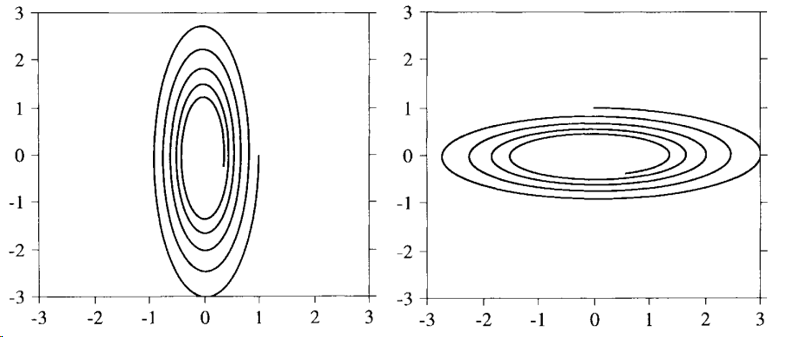
\includegraphics[width = 1 \linewidth]{screenshot001}
	\caption{Các quỹ đạo của $x_1$, $x_2$ trong hai trường hợp: Hệ 1 có tọa độ ban đầu là $x=\m{1 & 0 & 0}^T$ (hình trái); Hệ 2 có tọa độ ban đầu là $x=\m{0 & 1 & 0}^T$ (hình phải).}
	\label{fig:screenshot001}
\end{figure}

\begin{figure}[h!]
	\centering
	
\includegraphics[width=0.5\linewidth]{screenshot003}
	\caption{Quỹ đạo nghiệm của hệ chuyển mạch với tọa độ ban đầu là $x_0 = \m{10^{-6} & 0 & 0}^T$}
	\label{fig:screenshot003}
\end{figure}
\end{vd}

\begin{vd}\label{}
Tương tự như trong ví dụ trước, ta xét một hệ chuyển mạch bao gồm hai hệ tuyến tính con có ma trận là:\\
$$
\begin{aligned}
E &=\left[\begin{array}{ccc}
1 & 0 & 0 \\
0 & 1 & 0 \\
0 & 0 & 0
\end{array}\right], \\
A_{1} &= {\left[\begin{array}{ccc}
-1.8930 & 0.5846 & 0 \\
0.6124 & -0.0992 & 0 \\
0 & 0 & 1
\end{array}\right] }, \   
A_{2}= {\left[\begin{array}{ccc}
0.1024 & -0.8879 & 0 \\  
0.0959 & -1.3974 & 0 \\
0 & 0 & 1
\end{array}\right] }.
\end{aligned} 
$$
Khi đó ta có cả hai hệ con là không ổn định, mặc dù vậy dưới quy luật chuyển mạch tuần hoàn
%
\begin{equation}\label{ql2}
\sigma(t) = 
\begin{cases}
&1 \mbox{ if } 2k \leq t < 2k+1, \ k \in \mathbb{N}, \\
&2 \mbox{ if } 2k+1 \leq t < 2k+2, \ k \in \mathbb{N}, 
\end{cases}
\end{equation}
%
thì hệ thống tổng là ổn định mũ như trong Hình \ref{fig:screenshot004}.

\begin{figure}[h!]
	\centering
	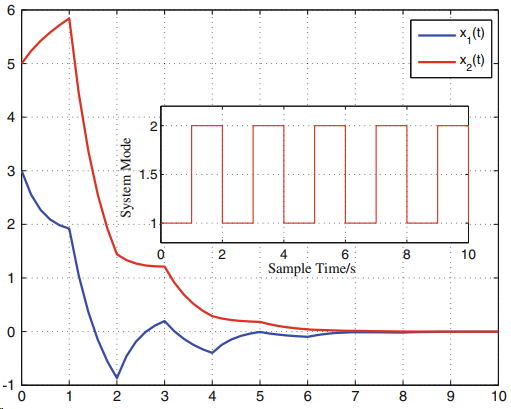
\includegraphics[width=0.7\linewidth]{screenshot004}
	\caption{Quỹ đạo nghiệm của hệ chuyển mạch với quy luật chuyển mạch \eqref{ql2}. }
	\label{fig:screenshot004}
\end{figure}
\end{vd}

Hai ví dụ trên đã minh họa cho hai bài toán cơ bản sau trong lý thuyết các hệ chuyển mạch, và được phát biểu dưới đây.

\begin{bt}\label{bài toán 1}
Giả  sử tất cả các hệ con trong \eqref{1.8} (hoặc \eqref{1.9}) là ổn định, hãy thiết lập điều kiện để hệ chuyển mạch \eqref{1.8} (hoặc \eqref{1.9}) ổn định dưới quy luật chuyển mạch tùy ý.
\end{bt}

\begin{bt}\label{bài toán 2}
Giả  sử có một hay nhiều hệ con trong hệ thống \eqref{1.8} (hoặc \eqref{1.9}) là không ổn định, hãy tìm điều kiện của hệ sao cho có thể thiết kế được một quy luật chuyển mạch thích hợp sao cho hệ thống \eqref{1.8} (hoặc \eqref{1.9}) là ổn định.
\end{bt}

Hai bài toán trên sẽ được nghiên cứu và giải quyết một phần trong Chương \ref{Chapter 2}.

%%%%%%%%%%%%%%%%%%%%%%%%%%%%%%%%%%%%%%%%%%%%%%%%%%%%%%%%%%%%%%%%%%%%%%%%%%%%%%%%%%%%%%%
%%%%%%%%%%%%%%%%%%%%%%%%%%%%%%%%%%%%%%%%%%%%%%%%%%%%%%%%%%%%%%%%%%%%%%%%%%%%%%%%%%%%%%%%%%%%%%%%%%%%%%%%%%%%%%%%%%%%%%%%%%%%%%%%%%%%%%%%%%%%%%%%%%%%%%%%%%%%%%%%%%%%%%%%%%%%%%
\chapter{Phân tích tính chất ổn định của các hệ chuyển mạch suy biến tuyến tính }\label{Chapter 2}
%%%%%%%%%%%%%%%%%%%%%%%%%%%%%%%%%%%%%%%%%%%%%%%%%%%%%%%%%%%%%%%%%%%%%%%%%%%%%%%%%%%%%%%%%%%%%%%%%%%%%%%%%%%%%%%%%%%%%%%%%%%%%%%%%%%%%%%%%%%%%%%%%%%%%%%%%%%%%%%%%%%%%%%%%%%%%%%%%%%%%%%%%%%%%%%%%%%%%%%%%%%%%%%%%%%%%%%%%%%%%%%%%%%%%%%%%%%%%%%%%%%%%%%%%%%%%%%%%%%%%
\section{Hệ trong miền thời gian liên tục với quy luật chuyển mạch tùy ý}
Trong phần này, trước tiên ta nêu ra và chứng minh điều kiện ổn định được mô tả bởi một số bất đẳng thức ma trận tuyến tính (LMIs). Kết quả này là một phần mở rộng không tầm thường của điều kiện ổn định giao hoán theo cặp.

\subsection{Điều kiện ổn định dựa trên LMIs}
\begin{dl}\label{dl2.1} Hệ chuyển mạch \eqref{1.8} là ổn định với quy luật chuyển mạch tùy ý nếu tồn tại ma trận $P_{i} \in \mathbb{R}^{n \times n}$ thỏa mãn
\begin{equation}
\begin{aligned}\label{2.1}
&E^{T} P_{i}=P_{i}^{T} E \geq 0 , 
\end{aligned} 
\end{equation}
\begin{equation}
\begin{aligned}\label{2.2}
&A_{i}^{T} P_{i}+P_{i}^{T} A_{i}<0  
\end{aligned} 
\forall i \in \mathcal{I}.
\end{equation}

Hơn nữa
\begin{equation}\label{2.3}
E^{T} P_{i}=E^{T} P_{j}, \quad \forall i, j \in \mathcal{I}, \quad i \neq j . 
\end{equation}
\end{dl}
\begin{cv} Các điều kiện \eqref{2.1} và \eqref{2.2} đảm bảo rằng mỗi hệ ổn định theo Định lí 1.2. Vì vậy, không khó để thấy rằng điều kiện\eqref{2.3} đề cập đến sự chuyển mạch từ hệ con thứ $i$ sang hệ con thứ $j$.

Vì hạng của $E$ là $r$, ta có thể tìm được hai ma trận khả nghịch $M$ và $N$ sao cho
\begin{equation}\label{2.4}
M E N=\left[\begin{array}{cc}
I_{r} & 0 \\
0 & 0
\end{array}\right]. 
\end{equation}
Từ \eqref{2.1} ta có
\begin{equation}\label{2.5}
N^{T} E^{T} M^{T}\left(M^{-1}\right)^{T} P_{i} N=N^{T} P_{i}^{T} M^{-1} M E N \geq 0. 
\end{equation}
Ta đặt
$$
\left(M^{-1}\right)^{T} P_{i} N:=\left[\begin{array}{cc}
P_{11}^{i} & P_{12}^{i} \\
P_{21}^{i} & P_{22}^{i}
\end{array}\right].
$$
Và ta có
\begin{equation} \label{2.6}
\begin{gathered}
{\left[\begin{array}{cc}
I_{r} & 0 \\
0 & 0
\end{array}\right]\left[\begin{array}{cc}
P_{11}^{i} & P_{12}^{i} \\
P_{21}^{i} & P_{22}^{i}
\end{array}\right]} =\left[\begin{array}{cc}
(P_{11}^{j})^T & (P_{12}^{i})^T \\
(P_{21}^{j})^T & (P_{22}^{j})^T
\end{array}\right]\left[\begin{array}{cc}
I_{r} & 0 \\
0 & 0
\end{array}\right] \geq 0. 
\end{gathered}
\end{equation}
Điều này dẫn đến $\left(P_{11}^{i}\right)^{T}=P_{11}^{i} \geq 0, P_{12}^{i}=0$. Do đó
\begin{equation}\label{2.7}
\left(M^{-1}\right)^{T} P_{i} N=\left[\begin{array}{cc}
P_{11}^{i} & 0 \\
P_{21}^{i} & P_{22}^{i}
\end{array}\right].
\end{equation}
Hơn thế nữa, từ \eqref{2.2} ta thấy rằng $P_{i}$ phải là khả nghịch. Ta chứng minh bằng phản chứng: Nếu $P_{i}$ không khả nghịch thì tồn tại $x \neq 0$ sao cho $P_{i} x=0$, dẫn đến $x^{T}\left(A_{i}^{T} P_{i}+P_{i}^{T} A_{i}\right) x=0$. Điều này mâu thuẫn với \eqref{2.2}. 

Vì $M$ và $N$ khả nghịch nên $\left(M^{-1}\right)^{T} P_{i} N$ cũng vậy, điều này nghĩa là $P_{11}^{i}$ và $P_{22}^{i}$ khả nghịch.

Tương tự, từ \eqref{2.3}, ta có
\begin{equation}\label{2.8}
N^{T} E^{T} M^{T}\left(M^{-1}\right)^{T} P_{i} N=N^{T} E^{T} M^{T}\left(M^{-1}\right)^{T} P_{j} N ,
\end{equation}
tương đương với
\begin{equation}\label{2.9}
\begin{gathered}
{\left[\begin{array}{cc}
I_{r} & 0 \\
0 & 0
\end{array}\right]\left[\begin{array}{cc}
P_{11}^{i} & 0 \\
P_{21}^{i} & P_{22}^{i}
\end{array}\right]}
=\left[\begin{array}{cc}
I_{r} & 0 \\
0 & 0
\end{array}\right]\left[\begin{array}{cc}
P_{11}^{j} & 0 \\
P_{21}^{j} & P_{22}^{j}
\end{array}\right] .
\end{gathered}
\end{equation}
Do đó $P_{11}^{i}=P_{11}^{j}, \forall i \neq j \in \mathcal{I}$, và ta viết lại \eqref{2.7} dưới dạng
\begin{equation}\label{2.10}
\left(M^{-1}\right)^{T} P_{i} N=\left[\begin{array}{cc}
P_{11} & 0 \\
P_{21}^{i} & P_{22}^{i}
\end{array}\right],
\end{equation}
trong đó $P_{11}$ là xác định dương và $P_{22}^{i}$ là khả nghịch.

Tiếp theo, phân rã
\begin{equation}\label{2.11}
M A_{i} N=:\left[\begin{array}{cc}
\bar{A}_{11}^{i} & \bar{A}_{12}^{i} \\
\bar{A}_{21}^{i} & \bar{A}_{22}^{i}
\end{array}\right]
\end{equation}
và thay thế nó vào \eqref{2.12}. Ta biến đổi  \eqref{2.2} về dạng tương đương
\begin{equation}\label{2.12}
N^{T} A_{i}^{T} M^{T}\left(M^{-1}\right)^{T} P_{i} N+N^{T} P_{i}^{T} M^{-1} M A_{i} N<0 
\end{equation}
để đạt được
\begin{equation}\label{2.13}
\left[\begin{array}{ll}
\Upsilon_{11} & \Upsilon_{12} \\
\Upsilon_{12}^{T} & \Upsilon_{22}
\end{array}\right]<0,
\end{equation}
trong đó
$$
\begin{aligned}
\Upsilon_{11}=&\left(\bar{A}_{11}^{i}\right)^{T} P_{11}+P_{11} \bar{A}_{11}^{i} 
+\left(\bar{A}_{21}^{i}\right)^{T} P_{21}^{i}+\left(P_{21}^{i}\right)^{T} \bar{A}_{21}^{i} \\
\Upsilon_{12}=&\left(\bar{A}_{21}^{i}\right)^{T} P_{22}^{i}+P_{11} \bar{A}_{12}^{i}+\left(P_{21}^{i}\right)^{T} \bar{A}_{22}^{i} \\
\Upsilon_{22}=&\left(\bar{A}_{22}^{i}\right)^{T} P_{22}^{i}+\left(P_{22}^{i}\right)^{T} \bar{A}_{22}^{i}
\end{aligned}
$$
\begin{equation}\label{2.14}
\left[\begin{array}{ll}I_{r} & 0 \\0 & 0\end{array}\right]\left[\begin{array}{ll}P_{11}^{i} & P_{12}^{i} \\P_{21}^{i} & P_{22}^{i}\end{array}\right] =\left[\begin{array}{ll}\left(P_{11}^{i}\right)^{T} & \left(P_{21}^{i}\right)^{T} \\\left(P_{12}^{i}\right)^{T} & \left(P_{22}^{i}\right)^{T}\end{array}\right]\left[\begin{array}{cc}I_{r} & 0 \\0 & 0\end{array}\right] \geq 0.
\end{equation}
Ta thấy rằng $\bar{A}_{22}^{i}$ không suy biến. \\
Phản chứng, giả sử tồn tại một vector $v$ khác $0$ sao cho $\bar{A}_{22}^{i} v=0$. Khi đó $v^{T} \Upsilon_{22} v<0$ do $\Upsilon_{22}<0$. Tuy nhiên, bằng phép tính
\begin{equation}\label{2.15}
v^{T} \Upsilon_{22} v=\left(\bar{A}_{22}^{i} v\right)^{T} P_{22}^{i} v+v^{T}\left(P_{22}^{i}\right)^{T}\left(\bar{A}_{22}^{i} v\right)=0
\end{equation}
dẫn đến sự mâu thuẫn.

Nhân từ bên trái của \eqref{2.14} với ma trận khả nghịch
$$
H=\left[\begin{array}{cc}
I_{r} & -\left(\bar{A}_{21}^{i}\right)^{T}\left(\left(\bar{A}_{22}^{i}\right)^{-1}\right)^{T} \\
0 & I_{n-r}
\end{array}\right]
$$
và từ bên phải của \eqref{2.14} với $H^T$, ta thu được
\begin{equation}\label{2.16}
\left[\begin{array}{cc}
\left(\tilde{A}_{11}^{i}\right)^{T} P_{11}+P_{11} \tilde{A}_{11}^{i} & * \\
\Upsilon_{12}^{T}-\Upsilon_{22}\left(\bar{A}_{22}^{i}\right)^{-1} \bar{A}_{21}^{i} & \Upsilon_{22}
\end{array}\right]<0, 
\end{equation}
trong đó $\tilde{A}_{11}^{i}=\bar{A}_{11}^{i}-\bar{A}_{12}^{i}\left(\bar{A}_{22}^{i}\right)^{-1} \bar{A}_{21}^{i}$.

Vì ma trận $E$ và $A_{i}$ được biến đổi tương ứng như trong \eqref{2.4} và \eqref{2.11}, ta đổi biến $\bar{x}:=$ $N^{-1} x=\left[\begin{array}{ll}\bar{x}_{1}^{T} & \bar{x}_{2}^{T}\end{array}\right]^{T}, \bar{x}_{1} \in \mathbb{R}^{r}$. Do đó, các hệ con trong \eqref{1.8} có dạng
\begin{equation}\label{2.17}
\begin{aligned}
\dot{\bar{x}}_{1} &=\bar{A}_{11}^{i} \bar{x}_{1}+\bar{A}_{12}^{i} \bar{x}_{2}, \\
0 &=\bar{A}_{21}^{i} \bar{x}_{1}+\bar{A}_{22}^{i} \bar{x}_{2},
\end{aligned} 
\end{equation}
tương đương với
\begin{equation}\label{2.18}
\dot{\bar{x}}_{1}=\left[\bar{A}_{11}^{i}-\bar{A}_{12}^{i}\left(\bar{A}_{22}^{i}\right)^{-1} \bar{A}_{21}^{i}\right] \bar{x}_{1}=\tilde{A}_{11}^{i} \bar{x}_{1},
\end{equation}
và
$$
\bar{x}_{2}=-\left(\bar{A}_{22}^{i}\right)^{-1} \bar{A}_{21}^{i} \bar{x}_{1}.
$$
Từ (2.16) ta thấy rằng
\begin{equation}\label{2.19}
\left(\tilde{A}_{11}^{i}\right)^{T} P_{11}+P_{11} \tilde{A}_{11}^{i}<0, 
\end{equation}
có nghĩa là tất cả $\tilde{A}_{11}^{i}$ là ổn định Hurwitz, và tồn tại ma trận  xác định dương $P_{11}$ chung cho tính ổn định của tất cả hệ con trong \eqref{2.18}. Do đó, $\bar{x}_{1}$ hội tụ về không theo cấp mũ dưới quy luật chuyển mạch tùy ý. Phần $\bar{x}_{2}$ bị chi phối bởi  $\bar{x}_{1}$ và do đó cũng hội tụ về không theo cấp số mũ. Điều này hoàn tất toàn bộ chứng minh.\qed \\
\end{cv}
\begin{nx}\label{Nx2} Khi $E=I$ và tất cả hệ con là ổn định Hurwitz, các điều kiện \eqref{2.1}-\eqref{2.3} phát biểu rằng có một ma trận xác định dương chung  $P$ thỏa mãn $A_{i}^{T} P+P A_{i}<0, \forall i \in \mathcal{I}$. Đây chính xác là điều kiện ổn định cho các hệ tuyến tính chuyển mạch  $\dot{x}(t)=A_{i} x(t)$ dưới quy luật  chuyển mạch tùy ý \cite{Nar94}. Do đó, Định lý \ref{dl2.1} là một mở rộng của kết quả hiện có cho các hệ không gian trạng thái tuyến tính chuyển mạch trong miền thời gian liên tục.\\
\end{nx} 

\begin{nx}\label{Nx3}  Từ chứng minh của Định lý \ref{dl2.1}, có thể thấy rằng $\bar{x}_{1}^{T} P_{11} \bar{x}_{1}$ là một hàm Lyapunov bậc hai chung cho tất cả hệ con của \eqref{2.18}. Do sự hội tụ theo cấp mũ của  $\bar{x}_{1}$ dẫn đến sự hội tụ của $\bar{x}_{2}$, ta có thể coi $\bar{x}_{1}^{T} P_{11} \bar{x}_{1}$ như là một hàm Lyapunov bậc hai chung cho toàn bộ hệ chuyển mạch. Thực tế, điều này là phù hợp bởi
%
\begin{align}\label{2.20}
x^{T} E^{T} P_{i} x &=\left(N^{-1} x\right)^{T}(M E N)^{T}\left(\left(M^{-1}\right)^{T} P_{i} N\right)\left(N^{-1} x\right)  \notag \\
&=\left[\begin{array}{c}
\bar{x}_{1} \\
\bar{x}_{2}
\end{array}\right]^{T}\left[\begin{array}{cc}
I_{r} & 0 \\
0 & 0
\end{array}\right]\left[\begin{array}{cc}
P_{11} & 0 \\
P_{21}^{i} & P_{22}^{i}
\end{array}\right]\left[\begin{array}{l}
\bar{x}_{1} \\
\bar{x}_{2}
\end{array}\right] \notag  \\
&=\bar{x}_{1}^{T} P_{11} \bar{x}_{1} .
\end{align} 
%
Do đó, mặc dù $E^{T} P_{i}$ và $V_{i}(x)=x^{T} E^{T} P_{i} x$ là không xác định dương, ta có thể coi $V_{i}(x)$ như một hàm Lyapunov bậc hai chung cho tất cả các  hệ con trong miền thời gian liên tục. Hơn nữa, nếu ta xét 
\begin{equation}\label{2.21}
V:=V_{\sigma(t)}(x) \triangleq x^{T} E^{T} P_{\sigma(t)} x,
\end{equation}
trong đó $\sigma(t)$ là chỉ số của hệ con kích hoạt tại $t$, như một dạng hàm Lyapunov cho hệ chuyển mạch, điều kiện \eqref{2.3} chỉ ra rằng không có hiện tượng nhảy giá trị khi xảy ra chuyển mạch. Điều này phù hợp với kết quả hiện có \cite{Br98} cho các hệ hỗn hợp và chuyển mạch chung.\\
\end{nx} 
\begin{nx}\label{Nx4}  Các điều kiện LMI \eqref{2.1}-\eqref{2.3} bao gồm một bất đẳng thức ma trận không ngặt có thể không dễ giải bằng cách sử dụng hộp công cụ điều khiển LMI hiện có trong Matlab. Trên thực tế, việc chứng minh Định lý \ref{dl2.1} đã gợi ý một phương pháp thay thế để giải nó trong một khuôn khổ các LMI ngặt như sau:

(i) Phân rã $E$ như trong \eqref{2.4} bằng cách sử dụng ma trận khả nghịch $M$ và $N$;

(ii) Tính $M A_{i} N$ với mọi $i \in \mathcal{I}$ như trong \eqref{2.11};

(iii) Giải các LMI nghiêm ngặt \eqref{2.13} với mọi $i \in \mathcal{I}$ đồng thời đối với $P_{11}>0, P_{21}^{i}$ và $P_{22}^{i}$;

(iv) Tính số $P_{i}$ ban đầu với
$$
P_{i}=M^{T}\left[\begin{array}{cc}
P_{11} & 0 \\
P_{21}^{i} & P_{22}^{i}
\end{array}\right] N^{-1}
$$
(dựa trên \eqref{2.10}).\\
\end{nx} 
\begin{nx}   Lưu ý rằng điều kiện \eqref{2.3} không nên được thay thế bằng điều kiện  $P_{i}=P_{j}, \forall i \neq j$. Lý do là việc thiết lập như vậy dẫn đến sự hạn chế của kết quả. Ví dụ, xét hệ chuyển mạch bao gồm hai hệ con có ma trận là
\begin{equation}\label{2.22}
\begin{aligned}
E &=\left[\begin{array}{cc}
I_{r} & 0 \\
0 & 0
\end{array}\right],
A_{1} &=\left[\begin{array}{cc}
-I_{r} & 0 \\
0 & I_{n-r}
\end{array}\right], A_{2}=\left[\begin{array}{cc}
-I_{r} & 0 \\
0 & -I_{n-r}
\end{array}\right].
\end{aligned}
\end{equation}
Dễ dàng kiểm tra rằng hệ chuyển mạch là ổn định tùy ý, nhưng ta không thể tìm thấy bất kỳ ma trận P thỏa mãn \eqref{2.2} cho cả  $A_{1}$ và $A_{2}$. Thật vậy, xét
$$
P=\left[\begin{array}{ll}
P_{11} & P_{12} \\
P_{21} & P_{22}
\end{array}\right]
$$
thì điều kiện \eqref{2.2} yêu cầu rằng
\begin{equation}\label{2.23}
\left[\begin{array}{cc}
-P_{11}-P_{11}^{T} & * \\
-P_{12}^{T}+P_{21} & P_{22}+P_{22}^{T}
\end{array}\right]<0 
\end{equation}
và
\begin{equation}\label{2.24}
\left[\begin{array}{cc}
-P_{11}-P_{11}^{T} & * \\
-P_{12}^{T}-P_{21} & -P_{22}-P_{22}^{T}
\end{array}\right]<0 .
\end{equation}
Tập trung vào khối (2,2) của ma trận ở vế trái, ta có thể dễ dàng thấy rằng hai bất đẳng thức trên không thể đồng thời được thỏa mãn.\\
Mặc dù trong trình bày vấn đề, ta giả định rằng ma trận mô tả$E$ là chung cho với mọi hệ con (như đã đề cập trong Nhận xét \ref{Nx1}), từ chứng minh của Định lí \ref{dl2.1}, ta chỉ thực sự cần điều kiện \eqref{2.4}. Do đó, Định lí \ref{dl2.1} có thể được mở rộng cho trường hợp như trong hệ quả sau đây.\\
\end{nx} 
\begin{corollary} \label{hq2.1} Xét hệ chuyển mạch bao gồm $\mathcal{N}$ hệ con được mô tả bởi 
\begin{equation}\label{2.25}
E_{i} \dot{x}(t)=A_{i} x(t),
\end{equation}
trong đó $E_{i}$ là ma trận mô tả của hệ con thứ $i$. Giả sử rằng tất cả các ma trận mô tả có cùng hạng $r$ và có các ma trận khả nghịch $M$ và $N$ sao cho 
\begin{equation}\label{2.26}
M E_{i} N=\left[\begin{array}{cc}
I_{r} & 0 \\
0 & 0
\end{array}\right], \quad \forall i \in \mathcal{I}. 
\end{equation}
Khi đó, hệ chuyển mạch \eqref{2.25} là ổn định dưới chuyển mạch tùy ý nếu tồn tại các ma trận $P_{i} \in \mathbb{R}^{n \times n} (i=1, \ldots, \mathcal{N})$ thỏa mãn với mọi $i \in \mathcal{I}$
\begin{equation}\label{2.27}
E_{i}^{T} P_{i}=P_{i}^{T} E_{i} \geq 0, \quad A_{i}^{T} P_{i}+P_{i}^{T} A_{i}<0,
\end{equation}
hơn nữa
\begin{equation}\label{2.28}
E_{i}^{T} P_{i}=E_{j}^{T} P_{j}, \quad \forall i, j \in \mathcal{I}, \quad i \neq j. 
\end{equation}
\end{corollary} 
\subsection{So sánh với điều kiện giao hoán theo cặp} Trong tiểu mục này, ta xét mối quan hệ của Định lí \ref{dl2.1} với kết quả trong \cite{Zhai09a}.\\

\begin{lemma} \label{bd2.1}\cite{Zhai09a} Nếu tất cả các hệ con ổn định và các ma trận $E, A_{1}, \ldots, A_{\mathcal{N}}$ giao hoán từng cặp, tức là\\
\begin{equation}\label{2.29}
E A_{i}=A_{i} E, \quad A_{i} A_{j}=A_{j} A_{i}, \quad \forall i, j \in \mathcal{I} \text {.} 
\end{equation}
Khi đó hệ chuyển mạch ổn định dướt quy luật chuyển mạch bất kỳ.
\end{lemma}
Bổ đề trên thiết lập một điều kiện đủ khác cho sự ổn định của hệ tuyến tính chuyển mạch trong điều kiện giao hoán theo cặp. Theo \cite{Nar94} trong trường hợp hệ tuyến tính chuyển mạch bao gồm các hệ con
\begin{equation}\label{2.30}
\dot{x}(t)=A_{i} x(t), \quad i \in \mathcal{I}, 
\end{equation}
trong đó tất cả hệ con là ổn định Hurwitz và các ma trận $A_{i}$ giao hoán theo cặp  ( tức là $\left(A_{i} A_{j}=A_{j} A_{i}, \forall i, j \in\right.$ $\mathcal{I}$ )thì tồn tại ma trận xác định dương P thỏa mãn 
\begin{equation}\label{2.31}
A_{i}^{T} P+P A_{i}<0.
\end{equation}
Sau đó, ta mong rằng nếu có điều kiện giao hoán của Bổ đề \ref{bd2.1} thì tồn tại một hàm Lyapunov bậc hai chung $V(x)=x^{T} E^{T} P_{i} x$ cho mọi hệ con và do đó thỏa mãn các điều kiện của Định lý \ref{dl2.1}. Điều này được phát biểu trong Định lý sau đây.\\


\begin{dl}\label{dl2.2}
Nếu tất cả các hệ con trong \eqref{1.8} là ổn định và các ma trận $E, A_{1}, \ldots, A_{\mathcal{N}}$ giao hoán theo từng  cặp, thì tồn tại các ma trận $P_{i} (i=$ $1, \ldots, \mathcal{N})$ thỏa mãn \eqref{2.1}-\eqref{2.3}. Do đó, hệ chuyển mạch ổn định dưới quy luật chuyển mạch bất kỳ.
\end{dl}


\begin{cv} Để đơn giản hóa về mặt ký hiệu, ta chỉ chứng minh trường hợp  $\mathcal{N}=2$. Do $\left(E, A_{1}\right)$ ổn định, theo Bổ đề \ref{bd1.1}, tồn tại hai ma trận khả nghịch $M, N$ sao cho
\begin{equation}\label{2.32}
\begin{gathered}
M E N=\left[\begin{array}{cc}
I_{r} & 0 \\
0 & 0
\end{array}\right], \\
M A_{1} N=\left[\begin{array}{cc}
\Lambda_{1} & 0 \\
0 & I_{n-r}
\end{array}\right],
\end{gathered} 
\end{equation}
trong đó $\Lambda_{1}$ là ma trận ổn định Hurwitz. Để không gây nhầm lẫn thì ở đây ta dùng ký hiệu  $M, N$ như phần trước.

Đặt
\begin{equation}\label{2.33}
N^{-1} M^{-1}:=\left[\begin{array}{ll}
W_{1} & W_{2} \\
W_{3} & W_{4}
\end{array}\right] 
\end{equation}
và thay nó vào điều kiện giao hoán $E A_{1}=$ $A_{1} E$ được viết lại dưới dạng
\begin{equation}\label{2.34}
\begin{aligned}
&(M E N)\left(N^{-1} M^{-1}\right)\left(M A_{1} N\right) =\left(M A_{1} N\right)\left(N^{-1} M^{-1}\right)(M E N),
\end{aligned} 
\end{equation}
ta có
\begin{equation}\label{2.35}
\left[\begin{array}{cc}
W_{1} \Lambda_{1} & W_{2} \\
0 & 0
\end{array}\right]=\left[\begin{array}{cc}
\Lambda_{1} W_{1} & 0 \\
W_{3} & 0
\end{array}\right].
\end{equation}
Do đó $W_{1} \Lambda_{1}=\Lambda_{1} W_{1}, W_{2}=0, W_{3}=0$.

Ta phân rã
\begin{equation}\label{2.36}
M A_{2} N=:\left[\begin{array}{cc}
\Lambda_{2} & X_{1} \\
X_{2} & X
\end{array}\right] 
\end{equation}
Theo điều kiện giao hoán $E A_{2}=$ $A_{2} E$, ta có
\begin{equation}\label{2.37}
\left[\begin{array}{cc}
W_{1} \Lambda_{2} & W_{1} X_{1} \\
0 & 0
\end{array}\right]=\left[\begin{array}{cc}
\Lambda_{2} W_{1} & 0 \\
X_{2} W_{1} & 0
\end{array}\right]. 
\end{equation}
Do đó $W_{1} \Lambda_{2}=\Lambda_{2} W_{1}, W_{1} X_{1}=0, X_{2} W_{1}=0$. Vì $N$, $ M$ không suy biến và  $W_{2}=0, W_{3}=0, W_{1}$ phải không suy biến. Ta thu được $X_{1}=0, X_{2}=0$. Hơn nữa, vì $\left(E, A_{2}\right)$ ổn định, $\Lambda_{2}$ là ổn định Hurwitz và $X$ phải không suy biến.\\

Điều kiện giao hoán thứ ba $A_{1} A_{2}=A_{2} A_{1}$ dẫn đến
\begin{equation}\label{2.38}
\left[\begin{array}{cc}
\Lambda_{1} W_{1} \Lambda_{2} & 0 \\
0 & W_{4} X
\end{array}\right]=\left[\begin{array}{cc}
\Lambda_{2} W_{1} \Lambda_{1} & 0 \\
0 & X W_{4}
\end{array}\right] .
\end{equation}
Ta có $\Lambda_{1} W_{1} \Lambda_{2}=\Lambda_{2} W_{1} \Lambda_{1}$. Kết hợp điều này với $W_{1} \Lambda_{1}=\Lambda_{1} W_{1}, W_{1} \Lambda_{2}=\Lambda_{2} W_{1}$, ta thu được
\begin{equation}\label{2.39}
W_{1} \Lambda_{1} \Lambda_{2}=\Lambda_{1} W_{1} \Lambda_{2}=\Lambda_{2} W_{1} \Lambda_{1}=W_{1} \Lambda_{2} \Lambda_{1},
\end{equation}
dẫn đến $\Lambda_{1}$ và $\Lambda_{2}$ giao hoán $\left(\Lambda_{1} \Lambda_{2}=\right.$ $\left.\Lambda_{2} \Lambda_{1}\right)$.

Tóm tắt lại, ta có
\begin{equation}\label{2.40}
M A_{2} N=\left[\begin{array}{cc}
\Lambda_{2} & 0 \\
0 & X
\end{array}\right] ,
\end{equation}
trong đó $\Lambda_{2}$ là ổn định Hurwitz, $X$ không suy biến và $\Lambda_{1} \Lambda_{2}=\Lambda_{2} \Lambda_{1}$. Theo kết quả từ \cite{Nar94}, tồn tại một ma trận xác định dương $P_{11}$ thỏa mãn $\Lambda_{i}^{T} P_{11}+P_{11} \Lambda_{i}<0, i=1,2$. 
Đặt
\begin{equation}\label{2.41}
\begin{aligned}
&P_{1}=M^{T}\left[\begin{array}{cc}
P_{11} & 0 \\
0 & -I_{n-r}
\end{array}\right] N^{-1}, \\
&P_{2}=M^{T}\left[\begin{array}{cc}
P_{11} & 0 \\
0 & -X
\end{array}\right] N^{-1},
\end{aligned}
\end{equation}
ta có
\begin{equation}\label{2.42}
(M E N)^{T}\left(\left(M^{-1}\right)^{T} P_{1} N\right)=\left[\begin{array}{cc}
P_{11} & 0 \\
0 & 0
\end{array}\right] \geq 0 
\end{equation}
và
\begin{equation}\label{2.43}
\begin{aligned}
&\left(M A_{1} N\right)^{T}\left(\left(M^{-1}\right)^{T} P_{1} N\right) +\left(\left(M^{-1}\right)^{T} P_{1} N\right)^{T}\left(M A_{1} N\right)\\ &\quad=\left[\begin{array}{cc}
\Lambda_{1}^{T} P_{11}+P_{11} \Lambda_{1} & 0 \\
0 & -I_{n-r}
\end{array}\right]<0 ,\\
&\left(M A_{2} N\right)^{T}\left(\left(M^{-1}\right)^{T} P_{2} N\right) +\left(\left(M^{-1}\right)^{T} P_{2} N\right)^{T}\left(M A_{2} N\right)\\
&\quad=\left[\begin{array}{cc}
\Lambda_{2}^{T} P_{11}+P_{11} \Lambda_{2} & 0 \\
0 & -X^{T} X
\end{array}\right]<0 .
\end{aligned}
\end{equation}
Do $P_{11}$ là chung cho $i=1,2$ và $N$ là khả nghịch, \eqref{2.42} và \eqref{2.43} chỉ ra rằng ma trận trong \eqref{2.41} thỏa mãn điều kiện \eqref{2.1}-\eqref{2.3}.
\qed
\end{cv}
%%%%%%%%%%%%%%%%%%%%%%%%%%%%%%%%%%%%%%%%%%%%%%%%%%%%%%%%%%%%%%%%%%%%%%%%%%%%%%%%%%%%%%
\section{Hệ trong miền thời gian rời rạc với quy luật chuyển mạch tùy ý}
Trong mục này ta phát biểu và chứng minh các kết quả tương tự như trong mục trước cho tính ổn định của hệ chuyển mạch với thời gian rời rạc trong \eqref{1.9} 
\begin{dl}\label{dl2.3} Hệ chuyển mạch \eqref{1.9} ổn định dưới quy luật chuyển mạch tùy ý nếu tồn tại các ma trận đối xứng khả nghịch $P_{i} \in \mathbb{R}^{n \times n}$ thỏa mãn với mọi $i \in \mathcal{I}$
\begin{equation}\label{2.44}
E^{T} P_{i} E \geq 0 ,
\end{equation}
\begin{equation}\label{2.45}
\begin{aligned}
& A_{i}^{T} P_{i} A_{i}-E^{T} P_{i} E<0,
\end{aligned} 
\end{equation}
và
\begin{equation}\label{2.46}
E^{T} P_{i} E=E^{T} P_{j} E, \quad \forall i, j \in \mathcal{I}, i \neq j.
\end{equation}
\end{dl}
\begin{cv} Tương tự như trong phần chứng minh của Định lý \ref{dl2.1}, các điều kiện \eqref{2.44}, \eqref{2.45} đảm bảo rằng mỗi hệ là ổn định \cite{Xu99}, trong khi đó điều kiện \eqref{2.46} giải quyết việc chuyển mạch hệ con thứ $i$ sang thứ $j$.\\

Do hạng của $E$ là $r$, đầu tiên ta tìm ma trận khả nghịch $M$ và $N$ sao cho ta có \eqref{2.4}. Từ \eqref{2.44} ta có
\begin{equation}\label{2.47}
N^{T} E^{T} M^{T}\left(M^{-1}\right)^{T} P_{i} M^{-1} M E N
\begin{aligned}
& =\left[\begin{array}{cc}P_{11}^{i} & 0 \\0 & 0\end{array}\right] \geq 0,
\end{aligned} 
\end{equation}
trong đó 
\begin{equation}\label{2.48}
\quad\left(M^{-1}\right)^{T} P_{i} M^{-1} \triangleq\left[\begin{array}{ccc}
P_{11}^{i} & P_{12}^{i} \\
\left(P_{12}^{i}\right)^{T} & P_{22}^{i}
\end{array}\right]. 
\end{equation}
Do $P_{i}$ đối xứng và khả nghịch, ta có $\left(M^{-1}\right)^{T} P_{i} M^{-1}$ 
 cũng đối xứng và khả nghịch. Vì vậy  $P_{11}^{i}>0$. \\
Từ \eqref{2.46} ta có 
\begin{equation}\label{2.49}
N^{T} E^{T} M^{T}\left(M^{-1}\right)^{T} P_{i} M^{-1} M E N \\
    = N^{T} E^{T} M^{T}\left(M^{-1}\right)^{T} P_{j} M^{-1} M E N, \
\end{equation}
và do đó $P_{11}^{i}=P_{11}^{j} \quad \forall i, j \in \mathcal{I}$. Vì vậy, ta cho  $P_{11}^{i}=P_{11}$  để đơn giản hóa ký hiệu.  \\
Xét phân rã $M A_i N$ như trong \eqref{2.11} và thay thế nó trong bất đẳng thức tương đương của \eqref{2.45} như sau
\begin{equation}\label{2.50}
N^{T} A_{i}^{T} M^{T} (M^{-1})^T P_i M^{-1} M A_i N \\
    - N^{T} E^{T} M^{T}\left(M^{-1}\right)^{T} P_{i} M^{-1} M E N < 0 
\end{equation}
ta thu được
\begin{equation}\label{2.51}
\left[\begin{array}{ccc}
\Lambda_{11} & \Lambda_{12} \\
\Lambda_{12}^{T} & \Lambda_{22}
\end{array}\right] <0 ,
\end{equation}
trong đó
\begin{equation}\label{2.52}
\begin{aligned}
\Lambda_{11}=&\left(\bar{A}_{11}^{i}\right)^{T} P_{11} \bar{A}_{11}^{i}-P_{11}+\left(\bar{A}_{21}^{i}\right)^{T}\left(P_{12}^{i}\right)^{T} \bar{A}_{11}^{i}\\
&+\left(\bar{A}_{11}^{i}\right)^{T} P_{12}^{i} \bar{A}_{21}^{i}+\left(\bar{A}_{21}^{i}\right)^{T} P_{22}^{i} \bar{A}_{21}^{i} \\
\Lambda_{12}=(&\left(\bar{A}_{11}^{i}\right)^{T} P_{11} \bar{A}_{12}^{i}+\left(\bar{A}_{11}^{i}\right)^{T} P_{12}^{i} \bar{A}_{22}^{i} \\
&+\left(\bar{A}_{21}^{i}\right)^{T}\left(P_{12}^{i}\right)^{T} \bar{A}_{12}^{i}+\left(\bar{A}_{21}^{i}\right)^{T} P_{22}^{i} \bar{A}_{22}^{i} \\
\Lambda_{22}=&\left(\bar{A}_{12}^{i}\right)^{T} P_{11} \bar{A}_{12}^{i}+\left(\bar{A}_{22}^{i}\right)^{T}\left(P_{12}^{i}\right)^{T} \bar{A}_{12}^{i} \\
&+\left(\bar{A}_{12}^{i}\right)^{T} P_{12}^{i} \bar{A}_{22}^{i}+\left(\bar{A}_{22}^{i}\right)^{T} P_{22}^{i} \bar{A}_{22}^{i}.
\end{aligned} 
\end{equation}
Ta kết luận rằng $\bar{A}_{22}^{i}$ là không suy biến vì  $\Lambda_{22}<0$. Phản chứng, giả sử có một vecto $v$ sao cho $\bar{A}_{22}^{i} v=0$. Khi đó, $v^{T} \Lambda_{22} v<0$. Tuy nhiên, bằng phép tính
\begin{equation}\label{2.53}
v^{T} \Lambda_{22} v=v^{T}\left(\bar{A}_{12}^{i}\right)^{T} P_{11} \bar{A}_{12}^{i} v \geq 0 
\end{equation}
Do $P_{11}$ xác định dương. Điều này dẫn đến sự mâu thuẫn.\\
Tương tự như trong chứng minh của Định lý \ref{dl2.1}, nhân trái \eqref{2.51} với 

$$
K= \left[\begin{array}{cc}
I_{r} & -\left(\bar{A}_{21}^{i}\right)^{T}\left(\left(\bar{A}_{22}^{i}\right)^{-1}\right)^{T} \\
0 & I_{n-r}
\end{array}\right]
$$
và nhân phải với $K^T$, ta thu được
\begin{equation}\label{2.54}
\left[\begin{array}{cc}
\left(\tilde{A}_{11}^{i}\right)^{T} P_{11} \tilde{A}_{11}^{i}-P_{11} & * \\
\Lambda_{12}^{T}-\Lambda_{22}\left(\bar{A}_{22}^{i}\right)^{-1} \bar{A}_{21}^{i} & \Lambda_{22}
\end{array}\right]<0 
\end{equation}
trong đó $\tilde{A}_{11}^{i}= \bar{A}_{11}^{i}-\bar{A}_{12}^{i}(\bar{A}_{22}^{i})^{-1} \bar{A}_{21}^{i}$.\\
Với cùng một phép biến đổi  $\bar{x}(k)=$ $N^{-1} x(k)=\left[\begin{array}{ll}\bar{x}_{1}^{T}(k) & \bar{x}_{2}^{T}(k)\end{array}\right]^{T}, \bar{x}_{1}(k) \in \mathbb{R}^{r}$, các hệ con trong \eqref{1.9} có dạng 
\begin{equation}\label{2.55}
\begin{aligned}
\bar{x}_{1}(k+1) &=\bar{A}_{11}^{i} \bar{x}_{1}(k)+\bar{A}_{12}^{i} \bar{x}_{2}(k), \\
0 &=\bar{A}_{21}^{i} \bar{x}_{1}(k)+\bar{A}_{22}^{i} \bar{x}_{2}(k),
\end{aligned} 
\end{equation}
tương đương với
\begin{equation}\label{2.56}
\bar{x}_{1}(k+1)=\tilde{A}_{11}^{i} \bar{x}_{1}(k) 
\end{equation}
và $\bar{x}_{2}(k)=-\left(\bar{A}_{22}^{i}\right)^{-1} \bar{A}_{21}^{i} \bar{x}_{1}(k)$.

Ngoài ra, từ \eqref{2.54}, ta thấy rằng
\begin{equation}\label{2.57}
\left(\tilde{A}_{11}^{i}\right)^{T} P_{11} \tilde{A}_{11}^{i}-P_{11}<0, \
\end{equation}
có nghĩa là tất cả các ma trận $\tilde{A}_{11}^{i}$ ổn định Schur, và tồn tại một ma trận xác định dương chung $P_{11}$ cho tính ổn định của tất cả các hệ con trong \eqref{2.56}. Do đó, $\bar{x}_{1}(k)$ hội tụ về không theo cấp mũ dưới quy luật chuyển mạch tùy ý. $\bar{x}_{2}(k)$ bị chi phối bởi $\bar{x}_{1}(k)$ do đó cũng hội tụ về 0 theo cấp mũ.\qed \\
\end{cv}
\begin{nx} Khi $E=I$ và tất cả hệ con ổn định Schur, điều kiện của Định lý \ref{dl2.3} thực sự yêu cầu một ma trận xác định dương chung $P$  thỏa mãn $A_{i}^{T} P A_{i}-P<0, \forall i \in \mathcal{I}$. Đây chính là điều kiện ổn định  cho hệ tuyến tính chuyển mạch dạng $x(k+1)=A_{i} x(k)$ dưới quy luật chuyển mạch tùy ý \cite{Nar94}. Do đó, Định lý \ref{dl2.3} là một mở rộng của kết quả hiện có cho các hệ chuyển mạch trong miền thời gian rời rạc.
\end{nx}
\begin{nx} Từ chứng minh của Định lý \ref{dl2.2} có thể thấy  $\bar{x}_{1}^{T} P_{11} \bar{x}_{1}$ là một hàm Lyapunov bậc hai chung cho tất cả các hệ con trong \eqref{2.56}. Như trong Nhận xét \ref{Nx3}, do sự hội tụ theo cấp mũ của $\bar{x}_{1}$ dẫn đến sự hội tụ của $\bar{x}_{2}$, ta có thể coi $\bar{x}_{1}^{T} P_{11} \bar{x}_{1}$ như một hàm Lyapunov bậc hai chung cho toàn bộ hệ chuyển mạch. Thực tế, điều này được thấy từ đẳng thức sau
\begin{equation}\label{2.58}
\begin{aligned}
x^{T} E^{T} P_{i} E x &=\left(N^{-1} x\right)^{T}(M E N)^{T}\left(\left(M^{-1}\right)^{T} P_{i} M^{-1}\right) \times(M E N)\left(N^{-1} x\right) \\
&=\left[\begin{array}{c}
\bar{x}_{1} \\
\bar{x}_{2}
\end{array}\right]^{T}\left[\begin{array}{cc}
I_{r} & 0 \\
0 & 0
\end{array}\right]\left[\begin{array}{cc}
P_{11} & P_{12}^{i} \\
\left(P_{12}^{i}\right)^{T} & P_{22}^{i}
\end{array}\right]  \times\left[\begin{array}{cc}
I_{r} & 0 \\
0 & 0
\end{array}\right]\left[\begin{array}{l}
\bar{x}_{1} \\
\bar{x}_{2}
\end{array}\right] \\
& =\bar{x}_{1}^{T} P_{11} \bar{x}_{1} .
\end{aligned} 
\end{equation}

Do đó, mặc dù $E^{T} P_{i} E$ và $V_{i}(x)=x^{T} E^{T} P_{i} E x$ không xác định dương, ta có thể coi $V_{i}(x)$ như một hàm Lyapunov bậc hai chung cho tất cả các hệ con trong miền thời gian rời rạc. Tương tự như trong Nhận xét \ref{Nx3}, nếu chúng ta coi \eqref{2.21} như một dạng hàm Lyapunov cho hệ chuyển mạch, điều kiện \eqref{2.46} chỉ ra rằng không có hiện tượng nhảy giá trị khi chuyển mạch xảy ra.
\end{nx}
Ta cũng nêu kết quả tương tự với Hệ quả \ref{hq2.1} và Định lý \ref{dl2.2}, bỏ qua phần chứng minh vì chứng minh tương tự như trong trường hợp thời gian liên tục.\\ 

\begin{corollary}\label{hq2.2} Xét một hệ chuyển mạch bao gồm $\mathcal{N}$ hệ con:
\begin{equation}\label{2.59}
E_{i} x(k+1)=A_{i} x(k) 
\end{equation}
trong đó $E_{i}$ là ma trận mô tả của hệ con thứ $i$. Giả sử rằng ma trận mô tả cũng có hạng $r$ và có ma trận khả nghịch chung $M$ và $N$ sao cho \eqref{2.26} thỏa mãn. Khi đó hệ chuyển mạch \eqref{2.59} ổn định dưới chuyển mạch tùy ý nếu có các ma trận đối xứng, khả nghịch $P_{i} \in \mathbb{R}^{n \times n} (i=1, \ldots, \mathcal{N})$ thỏa mãn với mọi $i \in \mathcal{I}$
\begin{equation}\label{2.60}
E_{i}^{T} P_{i} E_{i} \geq 0,\ A_{i}^{T} P_{i} A_{i}-E_{i}^{T} P_{i} E_{i}<0 ,
\end{equation}
và
\begin{equation}\label{2.61}
E_{i}^{T} P_{i} E_{i}=E_{j}^{T} P_{j} E_{j}, \quad \forall i, j \in \mathcal{I}, \quad i \neq j.
\end{equation}
\end{corollary}
\begin{dl}\label{dl2.4} Nếu tất cả các hệ con trong \eqref{1.9} ổn định và các ma trận $E, A_{1}, \ldots, A_{\mathcal{N}}$ giao hoán từng cặp thì tồn tại các ma trận đối xứng không suy biến $P_{i} (i=1, \ldots, \mathcal{N})$ thỏa mãn \eqref{2.44} - \eqref{2.52}, do đó hệ chuyển mạch \eqref{1.9} ổn định dưới quy luật chuyển mạch tùy ý.
\end{dl}

%%%%%%%%%%%%%%%%%%%%%%%%%%%%%%%%%%%%%%%%%%%%%%%%%%%%%%%%%%%%%%%%%%%%%%%%%%%%%%%%%%%%%%%
\section{Ví dụ số.}

Trong mục này ta cung cấp một ví dụ đơn giản để minh họa kết quả chính.

\begin{vd} Xét một hệ chuyển mạch tuyến tính bao gồm hai hệ con có ma trận hệ số là
\begin{equation}\label{2.62}
\begin{aligned}
E &=\left[\begin{array}{rrr}
-2 & -5 & 3 \\
1 & 1 & 0 \\
0 & 1 & -1
\end{array}\right] \\
A_{1} &=\left[\begin{array}{rrr}
-7 & 4 & -12 \\
0 & -1 & 1 \\
2 & -1 & 3
\end{array}\right]  \\
A_{2} &=\left[\begin{array}{rrr}
1 & 7 & -7 \\
-1 & -1 & 0 \\
0 & -2 & 2
\end{array}\right]
\end{aligned}
\end{equation}
Lưu ý rằng các ma trận này không thỏa mãn điều kiện giao hoán từng cặp được yêu cầu trong Bổ đề \ref{bd2.1}. Do đó sự ổn định dưới quy luật chuyển mạch tùy ý không thể được đảm bảo bởi kết quả trong \cite{Zhai09a} hoặc các tài liệu tham khảo khác.\\

Để giải quyết các LMI không ngặt \eqref{2.1} và \eqref{2.2}, ta sử dụng quy trình được mô tả trong Nhận xét \ref{Nx4}. Với các ma trận khả nghịch
\begin{equation}\label{2.63}
\begin{aligned}
&M=\left[\begin{array}{rrr}
0 & 1 & 0 \\
0 & 0 & 1 \\
-1 & -2 & -3
\end{array}\right], 
&N=\left[\begin{array}{rrr}
2 & -1 & -1 \\
-1 & 1 & 1 \\
-1 & 0 & 1
\end{array}\right],
\end{aligned}
\end{equation}
Ta có ma trận mô tả $E$ được phân rã thỏa mãn \eqref{2.4}. Sau đó, ta đi giải quyết LMI  ngặt \eqref{2.13} cho $i=1,2$ đối với các ẩn số $P_{11}>0, P_{21}^{i}, P_{22}^{i}$ và tính toán số $P_{i}$ ban đầu.
Với
$$
P_{i}=M^{T}\left[\begin{array}{cc}
P_{11} & 0 \\
P_{21}^{i} & P_{22}^{i}
\end{array}\right] N^{-1}, 
$$
\begin{figure}[h!]
	\centering
	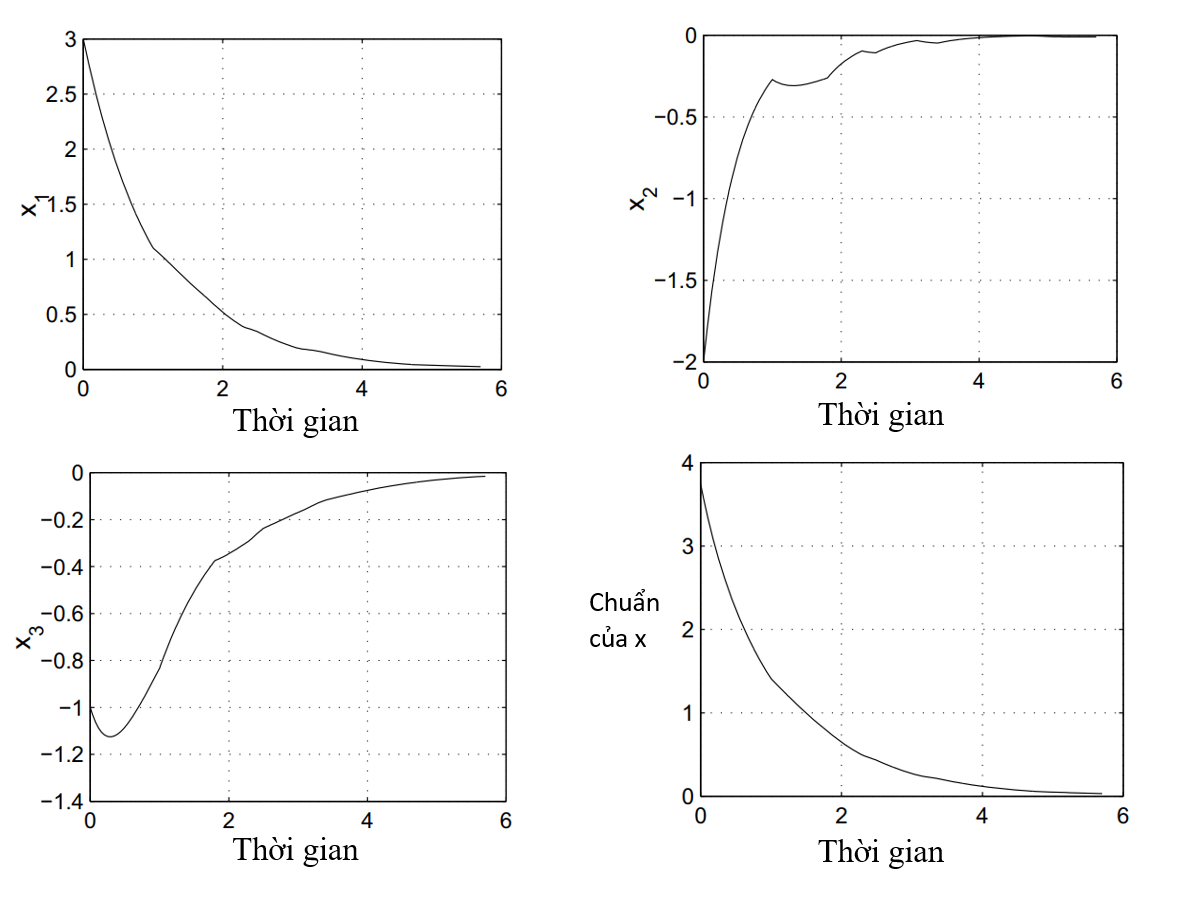
\includegraphics[width=1.0\linewidth]{Ảnh_LV.png}
	\caption{Các quỹ đạo của $x_{1}, x_{2}, x_{3}$ và sự hội tụ của $x$.\\}
\end{figure}

Ta đạt được
\begin{equation}\label{2.64}
\begin{aligned}
&P_{1}=\left[\begin{array}{rrr}
0.4344 & 0.1251 & 1.4708 \\
1.9914 & 1.1964 & 3.1180 \\
1.1268 & 0.5877 & 4.0235
\end{array}\right], \\ 
&P_{2}=\left[\begin{array}{rrr} 
1.7292 & 1.3588 & 2.6677 \\ 
4.5810 & 3.6638 & 5.5118 \\ 
5.0111 & 4.2888 & 7.6142
\end{array}\right].
\end{aligned}
\end{equation}
Ta thấy rằng các ma trận này thỏa mãn điều kiện \eqref{2.1} và \eqref{2.2}. Do đó, theo Định lý \ref{2.1}, hệ chuyển mạch ổn định dưới quy luật chuyển mạch tùy ý. \\
Trên thực tế, việc kích hoạt hai hệ thống luân phiên bằng một chuỗi thời gian được tạo ngẫu nhiên.\\
\begin{equation}\label{2.65}
1.0, 0.8, 0.5, 0.2, 0.6, 0.3, 1.4, 0.9, \ldots  
\end{equation}
(kích hoạt $\left(E, A_{1}\right)$ với khoảng thời gian $1.0$ và sau đó $\left(E, A_{2}\right)$ với khoảng thời gian $0.8$,\ldots ), quỹ đạo của hệ thống trạng thái (với trạng thái ban đầu $x_{0}=$ $\left.\left[\begin{array}{lll}3 & -2 & -1\end{array}\right]^{T}\right)$ và sự hội tụ theo chuẩn được thể hiện trong Hình 2.1. Rõ ràng, hệ chuyển mạch là ổn định.
\end{vd}
%%%%%%%%%%%%%%%%%%%%%%%%%%%%%%%%%%%%%%%%%%%%%%%%%%%%%%%%%%%%%%%%%%%%%%%%%%%%%%%%%%%%%
\section{Thiết kế quy luật chuyển mạch cho bài toán ổn định hóa}
Trong mục này chúng ta nghiên cứu bài toán thiết kế quy luật chuyển mạch để ổn định hóa hai hệ con
\begin{equation}\label{2}
  \begin{aligned}
  E \dot{x}(t)=A_{1} x, \\
   E \dot{x}(t)=A_{2} x, 
   \end{aligned}
\end{equation}
giả sử rằng hai hệ con trên đều không ổn định. 

Đối với hệ \eqref{2} với $E=I_{n}$ (mô hình không gian trạng thái), ta biết rằng nếu có một tổ hợp lồi của $A_{1}$ và $A_{2}$, tức là $\lambda A_{1}+(1-\lambda) A_{2} \quad(\lambda \in(0,1))$, là ổn định Hurrwitz, thì có một quy luật chuyển mạch để đạt được tính ổn định cho hệ chuyển mạch \cite{Br98}.

Ở đây, ta mở rộng ý tưởng về hệ tổ hợp lồi ổn định sang hệ chuyển mạch \eqref{2}, mặc dù hiện tại ta không xem xét tính ổn định bậc hai.
Ta giả định rằng cả hai hệ đều chính quy và không có xung. Theo Bổ đề \ref{bd1.1}, tồn tại hai ma trận không suy biến $M, N$ thỏa mãn 
\begin{equation} \label{3}
M^{-1}E N^{-1}=\left[\begin{array}{cc}I_{r} & 0 \\ 0 & 0\end{array}\right],\ M^{-1} A N^{-1}=\left[\begin{array}{cc}\Lambda_{1} & 0 \\ 0 & I_{n-r}\end{array}\right],  
\end{equation}
trong đó  $\Lambda_{1}$ không ổn định Hurwitz. Ta giả sử rằng $E, A_{1}, A_{2}$ giao hoán theo cặp, như được thực hiện trong phần trước, ta có: 
\begin{equation}\label{2.66}
M^{-1} A_{2} N^{-1}=\left[\begin{array}{cc}
\Lambda_{2} & 0 \\
0 & X
\end{array}\right] .
\end{equation}
Do $\left(E, A_{2}\right)$ không ổn định, $\Lambda_{2}$ không ổn định Hurwitz. $X$ khả nghịch vì $\left(E, A_{2}\right)$ không có xung.

Sau đó, ta xét một tổ hợp lồi của hai hệ như sau

\begin{equation}\label{2.67}
\left(E, A_{\lambda}\right) \triangleq\left(E, \lambda A_{1}+(1-\lambda) A_{2}\right) 
\end{equation}
trong đó $\lambda \in(0,1)$. Khi đó
\begin{equation}\label{2.68}
\begin{aligned}
& M^{-1} E N^{-1}=\left[\begin{array}{ll}
I_{r} & 0 \\
0 & 0
\end{array}\right] \\
& M^{-1} A_{\lambda} N^{-1}=\left[\begin{array}{cc}
\lambda \Lambda_{1}+(1-\lambda) \Lambda_{2} & 0 \\
0 & \lambda I+(1-\lambda) X
\end{array}\right]
\end{aligned} 
\end{equation}
Nếu ta có thể tìm thấy một vô hướng $\lambda \in(0,1)$ sao cho $\left(E, A_{\lambda}\right)$ ổn định, thì từ \eqref{2.68} ta có $\lambda \Lambda_{1}+(1-\lambda) \Lambda_{2}$ là ổn định (Hurwitz) và $\lambda I+(1-\lambda) X$ khả nghịch.

Do đó, tính ổn định của hệ chuyển mạch có thể được nghiên cứu cho hệ chuyển mạch 
$$
  \begin{aligned}
  \dot{\bar{x_1}}= \Lambda_{1} \bar{x_1}, \ \bar{x_2}=0
   \end{aligned}
$$
và
$$
\begin{aligned}
  \dot{\bar{x_1}}= \Lambda_{2} \bar{x_1}, \ X\bar{x_2}=0,
   \end{aligned}
$$
với phép đổi biến $\bar{x}=N x$. Phần $\bar{x}_{2}$ vẫn là không dù ta chuyển mạch thế nào. Liên quan đến phần $\bar{x}_{1}$, ta biết $\lambda \Lambda_{1}+(1-\lambda) \Lambda_{2}$ ổn định Hurwitz, và $\Lambda_{1}$ giao hoán với $\Lambda_{2}$. Ta đề xuất quy luật chuyển mạch sau.

\begin{ql} \label{ql1}
Kích hoạt hai hệ theo trình tự với các khoảng thời gian $\lambda T$ và $(1-\lambda) T$ tương ứng, trong đó T > 0 tùy ý.
\end{ql}

Vì $\Lambda_{\lambda} \triangleq \lambda \Lambda_{1}+(1-\lambda) \Lambda_{2}$ ổn định Hurwitz, và $\Lambda_{1}$ và $\Lambda_{2}$ không ổn định (Hurwitz), luôn tồn tại vô hướng dương $\alpha_{s}, \alpha_{u}$ và $k_{s}, k_{u}$ sao cho 
\begin{equation}\label{2.69}
\left\|e^{\Lambda_{\lambda} t}\right\| \leq k_{s} e^{-\alpha_{s} t}, \quad\left\|e^{\Lambda_{i} t}\right\| \leq k_{u} e^{\alpha_{u} t} \ (i=1,2) 
\end{equation}
với $\forall t \geq 0$. Với $t>0$ bất kỳ, ta chia khoảng $[0, t)$ theo luật chuyển mạch là $t=l T+\hat{t}$, trong đó $l$ là số nguyên không âm, $0 \leq \hat{t}<T$. Do $\Lambda_{1}$ và $\Lambda_{2}$ giao hoán, với bất kỳ điều kiện ban đầu $\bar{x}_{1}(0)$ nào, ta có
\begin{equation}\label{2.70}
\begin{aligned}
\left|\bar{x}_{1}(t)\right| & \leq k_{s} e^{-\alpha_{s}(l T)} \times k_{u} e^{\alpha_{u} \hat{t}}\left|\bar{x}_{1}(0)\right| \\
&=\left(k_{s} k_{u}\right) e^{-\alpha_{s}(l T+\hat{t})} \times e^{\left(\alpha_{s}+\alpha_{u}\right) t}\left|\bar{x}_{1}(0)\right| \\
& \leq\left(k_{s} k_{u} e^{\left(\alpha_{s}+\alpha_{u}\right) T}\right) e^{-\alpha_{s} t}\left|\bar{x}_{1}(0)\right|, 
\end{aligned} 
\end{equation}
kéo theo $\bar{x}_{1}$ hội tụ theo cấp mũ.

\begin{dl}\label{dl2.5} Giả sử rằng hai hệ trong \eqref{2}  không ổn định, và các ma trận  $E$,  $A_{1}, A_{2}$ giao hoán theo từng cặp. Nếu có một tổ hợp lồi ổn định $\left(E, A_{\lambda}\right)$ của hệ, thì hệ chuyển mạch \eqref{2} ổn định theo quy luật chuyển mạch \ref{ql1}.
\end{dl}
\begin{nx} \label{nx2.7} Định lý \ref{dl2.5} có thể mở rộng cho các hệ chuyển mạch bao gồm hơn hai hệ. Ví dụ: $E \dot{x}=A_{i} x, i=1, \dots, L$ thì tổ hợp lồi của hệ đang được xem xét có dạng $\left(E, \sum_{i=1}^{L} \lambda_{i} A_{i}\right)$, trong đó $\lambda_{i} \geq 0, \sum_{i=1}^{L} \lambda_{i}=1 .$
\end{nx}
Ta quan sát thấy rằng tính chất ổn định bây giờ được chuyển thành việc tìm một tổ hợp lồi ổn định $\left(E, A_{\lambda}\right)$. Đây nói chung là một nhiệm vụ rất khó khăn. Một phương pháp thực tế để tìm một tổ hợp như vậy là sử dụng điều kiện dựa trên bất đẳng thức ma trận được đề xuất trong \cite{E99}. Chính xác hơn, ta giới thiệu các ma trận $V, U \in R^{n \times(n-r)}$ có hạng cột đầy đủ và là hệ vector cơ sở của Null $E$, Null $E^{T}$ tương ứng. Khi đó, theo \cite{E99}, $\left(E, A_{\lambda}\right)$ ổn định khi và chỉ khi tồn tại ma trận xác định dương $P$ và ma trận $S \in R^{(n-r) \times(n-r)}$ thỏa mãn bất đẳng thức ma trận
\begin{equation}\label{2.71}
\begin{aligned}
&{\left[\lambda A_{1}+(1-\lambda) A_{2}\right]\left(P E^{T}+V S U^{T}\right)} \\
&+\left(P E^{T}+V S U^{T}\right)\left[\lambda A_{1}+(1-\lambda) A_{2}\right]<0 .
\end{aligned} 
\end{equation}
Do đó, vấn đề điều khiển được rút gọn thành giải \eqref{2.71} đối với $P>0, S$ và $0<\lambda<1$.

Điều kiện \eqref{2.71} là bất đẳng thức ma trận song tuyến tính (BMI) theo $\lambda$ và $(P, S)$. Như đã biết, giải quyết bài toán BMI không phải dễ dàng. Vì vậy một phương pháp tùy chỉnh cho $\lambda$ được thực hiện theo ý tưởng như sau. Vì bất đẳng thức ma trận \eqref{2.71} là "liên tục" đối với $\lambda$, chúng ta tách khoảng $(0,1)$ thành một chuỗi các giá trị $d_{1}, d_{2}, \dots, d_{K-1}$ với $d_{i}=\frac{i}{K}$ và $K$ đủ lớn, và giải bất đẳng thức ma trận tuyến tính \eqref{2.71} với $\lambda$ cố định là $d_{i}$, sử dụng phần mềm LMI hiện có. Nếu bất đẳng thức ma trận ban đầu là khả thi, chúng ta có thể mong đợi rằng phương pháp này hội tụ với một số $d_{i}$ khi sự tùy biến là đủ tốt (hoặc $K$ đủ lớn). Ta thấy rằng đây là một phương pháp hiệu quả trong nhiều trường hợp.

\begin{nx} Từ bất đẳng thức ma trận \eqref{2.71} rằng $\left(E, A_{\lambda}\right)$ ổn định khi và chỉ khi tồn tại $\lambda_{1} \geq 0$ và $\lambda_{2} \geq 0$ sao cho $\left(E, \lambda_{1} A_{1}\right.$ $\left.+\lambda_{2} A_{2}\right)$ ổn định. Do đó, tổ hợp lồi $\left(E, A_{\lambda}\right) \triangleq\left(E, \lambda A_{1}+(1-\lambda) A_{2}\right)$, trong đó $\lambda \in$ $(0,1)$, có thể được thay thế bằng tổ hợp dương $\left(E, A_{\lambda}\right) \triangleq\left(E, \lambda_{1} A_{1}+\lambda_{2} A_{2}\right)$, trong đó $\lambda_{1} \geq 0, \lambda_{2} \geq 0$. Điều này cũng đúng với trường hợp liên quan đến nhiều hơn ba hệ, như được mô tả trong Nhận xét \ref{nx2.7}. 
\end{nx}
Tiếp theo chúng ta sẽ thảo luận về điều kiện giao hoán. Quan sát thấy rằng điều kiện giao hoán giữa ma trận mô tả $E$ và các ma trận $A_{i}$  dẫn đến các dạng Weiertrass \eqref{3} và 
\begin{equation} \label{4}
 M^{-1} A_{2} N^{-1}=\left[\begin{array}{cc}\Lambda_{2} & 0 \\ 0 & X\end{array}\right]   
\end{equation}
và tính chất giao hoán của $\Lambda_{1}$ và $\Lambda_{2}$. Trong một số bài toán ứng dụng thực tế, điều kiện giao hoán có thể không được thỏa mãn, và do đó chúng ta nên xem xét khả năng nới lỏng điều kiện này.

Lưu ý rằng ngay cả khi điều kiện giao hoán không được thỏa mãn, \eqref{3} vẫn đúng vì $\left(E, A_{1}\right)$ là chính quy. Do đó, điều kiện giao hoán có thể được nới lỏng là: \emph{"với các ma trận khả nghịch $M$ và $N$, ma trận $A_{2}$ có dạng \eqref{4}."} Hơn nữa, ta thấy rằng  nếu
\begin{equation} \label{5}
   M^{-1} A_{2} N^{-1}=\left[\begin{array}{cc}
\Lambda_{2} & X_{1} \\
0 & X
\end{array}\right], 
\end{equation} 
trong đó $X_{1}$ không cần thiết phải bằng không, thì \eqref{2.68} trở thành 
$$
\begin{aligned}
M^{-1} E N^{-1} &=\left[\begin{array}{cc}
I_{r} & 0 \\
0 & 0
\end{array}\right], \\
M^{-1} A_{\lambda} N^{-1} &=\left[\begin{array}{cc}
\lambda \Lambda_{1}+(1-\lambda) \Lambda_{2} & X_{1} \\
0 & \lambda I+(1-\lambda) X
\end{array}\right].
\end{aligned} 
$$
Trong trường hợp này, điều kiện $\left(E, A_{\lambda}\right)$ ổn định kéo theo $\lambda \Lambda_{1}+(1-\lambda) \Lambda_{2}$ là ổn định Hurwitz và  $\lambda I+(1-\lambda) X$ khả nghịch. Mặc dù  $\Lambda_{1}$ và $\Lambda_{2}$ không giao hoán, theo tài liệu hiện có \cite{M98}, tồn tại một quy luật chuyển mạch phụ thuộc trạng thái để hệ chuyển mạch là ổn định.


\begin{corollary} Giả sử rằng hai hệ trong \eqref{2} là chính quy và không có xung, và $A_{2}$ có dạng như trong \eqref{5} với các ma trận khả nghịch $M$ và $N$ trong dạng Weiertrass \eqref{3} của $\left(E, A_{1}\right)$. Nếu có một tổ hợp lồi ổn định $\left(E, A_{\lambda}\right)$ của các hệ, thì tồn tại quy luật chuyển mạch để hệ chuyển mạch ổn định mũ.
\end{corollary}
\begin{nx}Mặc dù trong mục này chuáng ta chỉ chứng minh các kết quả cho trường hợp thời gian liên tục nhưng Quy luật chuyển mạch \ref{ql1} vẫn đúng trong trường hợp thời gian rời rạc.
\end{nx}
%%%%%%%%%%%%%%%%%%%%%%%%%%%%%%%%%%%%%%%%%%%%%%%%%%%%%%%%%%%%%%%%%%%%%%%%%%%%%%%%%%%%%
\chapter{Kết luận}

Trong luận văn này, một cách tiếp cận thống nhất để phân tích tính chất ổn định cho các hệ tuyến tính dưới quy luật chuyển mạch tùy ý được thiết lập trong cả hai trường hợp miền thời gian liên tục và miền thời gian rời rạc.
Chi tiết hơn, nếu có một hàm Lyapunov bậc hai chung cho tính ổn định của các hệ con thì hệ chuyển mạch ổn định dưới quy luật chuyển mạch tùy ý.
Hàm Lyapunov bậc hai chung được đề xuất là không xác định dương cho tất cả các trạng thái, nhưng chúng thực sự đóng vai trò của hàm Lyapunov như trong lý thuyết ổn định Lyapunov cổ điển. Cách tiếp cận trên là mở rộng tự nhiên của cách tiếp cận hiện có cho các hệ không gian trạng thái tuyến tính chuyển mạch.

Trong trường hợp không có hệ con nào là ổn định, dựa trên việc xem xét các tổ hợp lồi của các hệ con, ta vẫn có thể thiết kế được một quy luật chuyển mạch phù hợp để ổn định hóa hệ chuyển mạch. Đây là mở rộng tự nhiên và quan trọng của các hệ chuyển mạch không suy biến lên trường hợp các hệ chuyển mạch suy biến.

Các mục tiêu nghiên cứu xa hơn bao gồm: (1) Nghiên cứu sâu thêm về cấu trúc cặp ma trận của hệ để phân tích tính chất ổn định dưới quy luật chuyển mạch bất kỳ; (2) Giảm nhẹ điều kiện giao hoán trong việc thiết kế quy luật chuyển mạch phù hợp cho bài toán ổn định hóa.

\newpage
\setlength{\parskip}{0.3cm}
%\setlength{\headsep}{o cm}
\addcontentsline{toc}{chapter}{Kết Luận}

\begin{thebibliography}{99} % Tài liệu tham khảo
	\addcontentsline{toc}{chapter}{{\bf Tài liệu tham khảo}\rm}

\bibitem{Br98} 
Branicky, M.S., Multiple Lyapunov functions and other analysis tools for switched and hybrid systems, \emph{IEEE Transactions on Automatic Control}, 1998. 

\bibitem{LTW11} 
Daniel Liberzon, Stephan Trenn and Fabian Wirth, Commutativity and asymptotic stability for linear switched DAEs. \emph{2011 50th IEEE Conference on Decision and Control and European Control Conference (CDC-ECC) Orlando, FL, USA}, December 12-15, 2011.

\bibitem{Masu97} I. Masubuchi, Y. Kamitane, A. Ohara, and N. Suda, $\mathcal{H}_{\infty}$ control for descriptor systems: a matix inequalities approach  \emph{Automatica}, 1997.

\bibitem{Nar94} Narendra, K.S and Balakrishnan,J.. A common Lyapunov function for stable LTI systems with commuting A-matrices, \emph{IEEE Transactions on Automatic Control}, 1994.

\bibitem{E99} E. Uezato and M. Ikeda, Strict LMI conditions for stability, robust stabilization, and $\mathcal{H}_{\infty}$ control of descriptor systems, \emph{Proc. of the 38th IEEE Conference on Decision and Control}, Phoenix, USA 1999.

\bibitem{M98} M. A. Wicks, P. Peleties, and R. A. DeCarlo, Swithched controller design for the quadratic stabilization of a pair of unstable linear systems  \emph{European Journal of Control}, 1998.

\bibitem{Xu99} Xu, S. and Yang, C. .Stabilization of discrete-time singular systems: A matrix inequalities opproach, \emph{Automatica}, 1999.

\bibitem{Zhai09a} 
Guisheng Zhai, Ryuuen Kou, Joe Imae, and Tomoaki Kobayashi,	Stability Analysis and Design for Switched Descriptor Systems,  \emph{International Journal of Control, Automation, and Systems} (2009) 7(3):349-355.

\bibitem{Zhai10} Guisheng Zhai, Xuping Xu, A unified approach to stability analysis of switched linear descriptor symtems under arbitrary switching,	\emph{International Journal of Applied Mathematics and Computer Science}, 2010, Vol. 20, No. 2, 249–259.

\bibitem{book1} Dan Zhang, Li Yu, {\itshape Analysis and Synthesis of Switched Time-Delay Systems: The Average Dwell Time Approach}, Springer, 2019.


% 	\bibitem {1} \label{tltk1}
% 	W. Chen, C. Li, Y. Li; {\itshape A direct method of moving planes for the fractional Laplacian} , Adv. Math. 308 (2017) 404–437.
	
% 	\bibitem {2} \label{tltk2}
% 	W. Chen, C. Li, B. Ou; {\itshape Classification of solutions for an integral equation} , Comm. Pure Appl. Math. 59 (2006) 330–343.
	
% 	\bibitem {3} \label{tltk3}
% 	W. Dai, Y. Fang, J. Huang, Y. Qin, B. Wang; {\itshape Regularity and classification of solutions to static Hartree equations involving fractional Laplacians} , Discrete Contin. Dyn. Syst. Ser. A 38 (2018) 2795–2809.
	
% 	\bibitem {4} \label{tltk4}
% 	T. Kulczycki; {\itshape Properties of green function of symmetric stable processes} , Probab. Math. Stat. 17 (1997) 339–364.
	
% 	\bibitem {5} \label{tltk5}
% 	E. Lieb; {\itshape Sharp constants in the Hardy-Littlewood-Sobolev and related inequalities} , Ann. of Math. 118 (1983) 349–374.
	
% 	\bibitem {6} \label{tltk6}
% 	B. Ou; {\itshape A remark on a singular integral equation} , Houston J. Math. 25 (1999) 181–184.
	
% 	\bibitem {7} \label{tltk7}
% 	Phuong Le; {\itshape Liouville theorem and classification of positive solutions for a fractional Choquard type equation}, Nonlinear Anal. 185 (2019) 123-141.
	
% 	\bibitem {8} \label{tltk8}
% 	L. Silvestre; {\itshape Regularity of the obstacle problem for a fractional power of the Laplace operator} , Comm. Pure Appl. Math.
% 	60 (2007) 67–112.
	
	
% 	\bibitem {9} \label{tltk9}
% 	R. Zhuo, W. Chen, X. Cui, Z. Yuan; {\itshape A Liouville theorem for the fractional Laplacian}, preprint, arXiv:1401.7402.
\end{thebibliography}


\end{document}


